\pdfobjcompresslevel=1
%\documentclass[notes=only]{beamer}
\documentclass[notes=hide]{beamer}
\usetheme[titlepagelogo=img/cover]{LDN}

\usepackage[utf8]{inputenc}
\usepackage[francais]{babel}
\usepackage[T1]{fontenc}
\usepackage{tabularx, verbatim, xcolor}
\usepackage{lmodern, alltt, graphicx, ragged2e}
\usepackage{marvosym, multicol, textcomp, eurosym}

\definecolor{darkgreen}{RGB}{0,99,0}
\newcommand{\good}{{\color{green}\Smiley}}
\newcommand{\bad}{{\color{red}\Frowny}}

\date{\textbf{FSM 2015}}

\title{La Brique Internet}
\subtitle{\vspace{10pt}\emph{Internet Neutre \& Auto-Hébergement}}
\author{Neutrinet \\ Lorraine Data Network}
\begin{document}

\begin{frame}[t,plain]
\titlepage
\end{frame}

\watermarkon
\watermarkoff

\begin{frame}[t]{}
\begin{center}
\vfill
{\Huge \textbf{Nettoyer son accès à Internet}}
\vspace{.5cm}

{\large \emph{Juste en branchant un câble}}
\vspace{1cm}

\textbf{1 / 2}
\vfill
\end{center}
\end{frame}

\begin{frame}[t]{Je suis chez MachinTelecom}
\begin{center}
\vfill
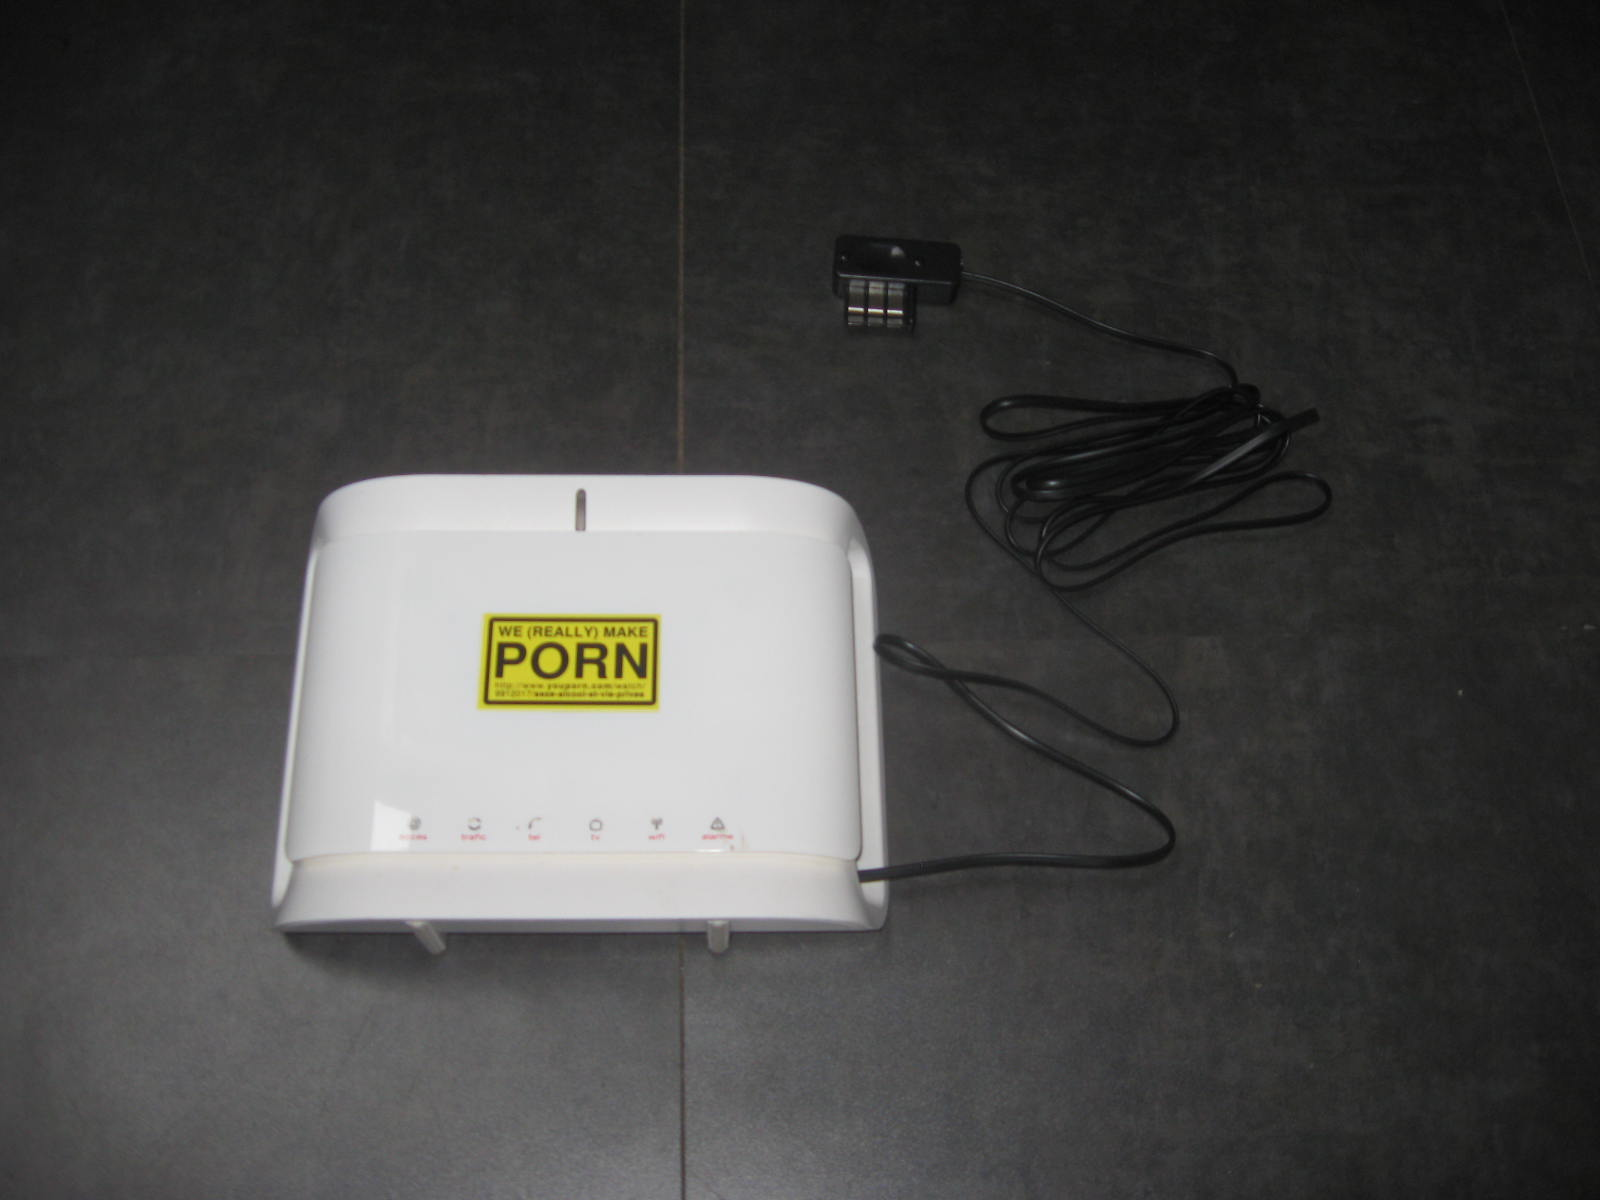
\includegraphics[width=.75\textwidth]{img/01-photo-neufbox.jpg}
\vfill
\end{center}
\end{frame}

\begin{frame}[t]{Je suis connecté au wifi de mon routeur}
\begin{center}
\vfill
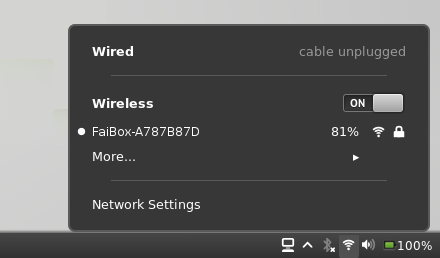
\includegraphics[width=.9\textwidth]{img/02-capture-wifibox.png}
\vfill
\end{center}
\end{frame}

\begin{frame}[t]{Mais je n'ai pas confiance en mon FAI}
\begin{center}
\vfill

\includegraphics[width=.75\textwidth]{img/03a-schema-connexionbox.pdf}
\vfill
\end{center}
\end{frame}

\begin{frame}[t]{... il peut espionner}
\begin{center}
\vfill

\includegraphics[width=.75\textwidth]{img/03b-schema-connexionbox.pdf}
\vfill
\end{center}
\end{frame}

\begin{frame}[t]{... il peut censurer}
\begin{center}
\vfill

\includegraphics[width=.75\textwidth]{img/03c-schema-connexionbox.pdf}
\vfill
\end{center}
\end{frame}

\begin{frame}[t]{... et il peut brider}
\begin{center}
\vfill

\includegraphics[width=.75\textwidth]{img/03d-schema-connexionbox.pdf}
\vfill
\end{center}
\end{frame}

\begin{frame}[t]{Mon FAI ne me donne aucune garantie}
\begin{center}
\vfill
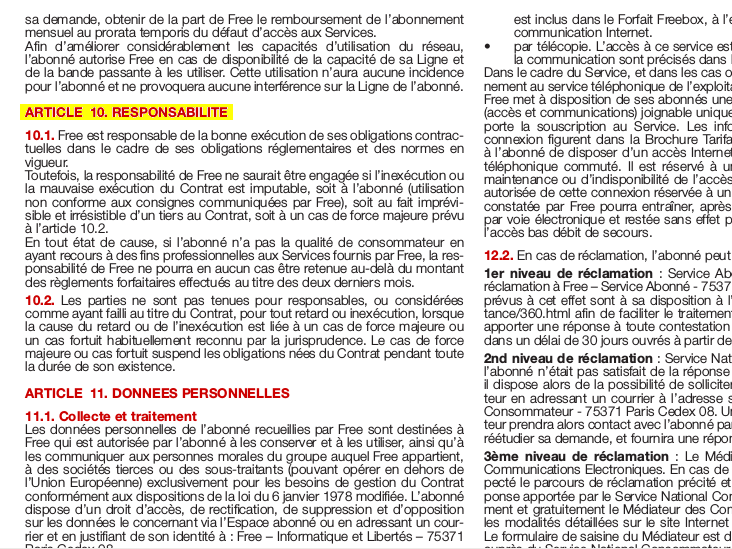
\includegraphics[width=.75\textwidth]{img/03f-cgu.png}
\vfill
\end{center}
\end{frame}

\begin{frame}[t]{Et promet de ne pas respecter ma vie privée}
\begin{center}
\vfill
\includegraphics[width=.75\textwidth]{img/03g-cgu.png}
\vfill
\end{center}
\end{frame}

\begin{frame}[t]{Une association m'a fourni une Brique Internet}
\begin{center}
\vfill
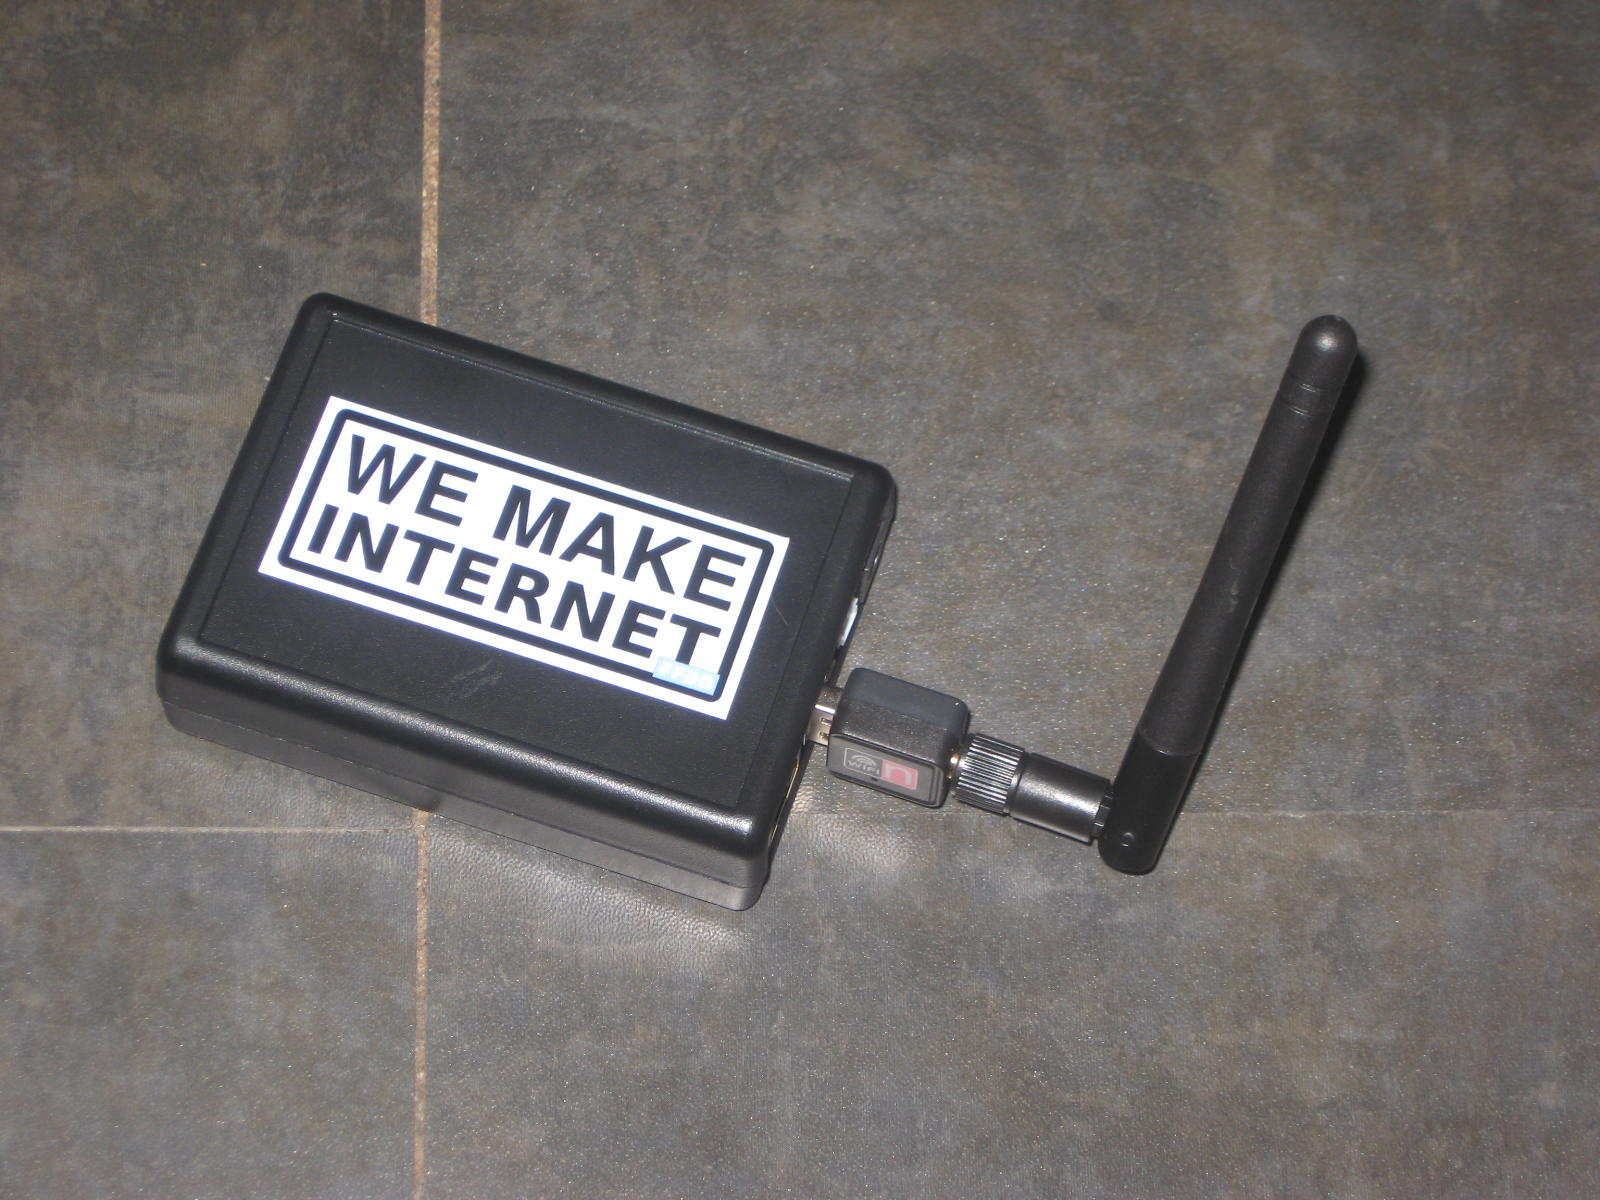
\includegraphics[width=.75\textwidth]{img/04-photo-boitier.jpg}
\vfill
\end{center}
\end{frame}

\begin{frame}[t]{Je n'ai qu'à la brancher à mon routeur}
\begin{center}
\vfill
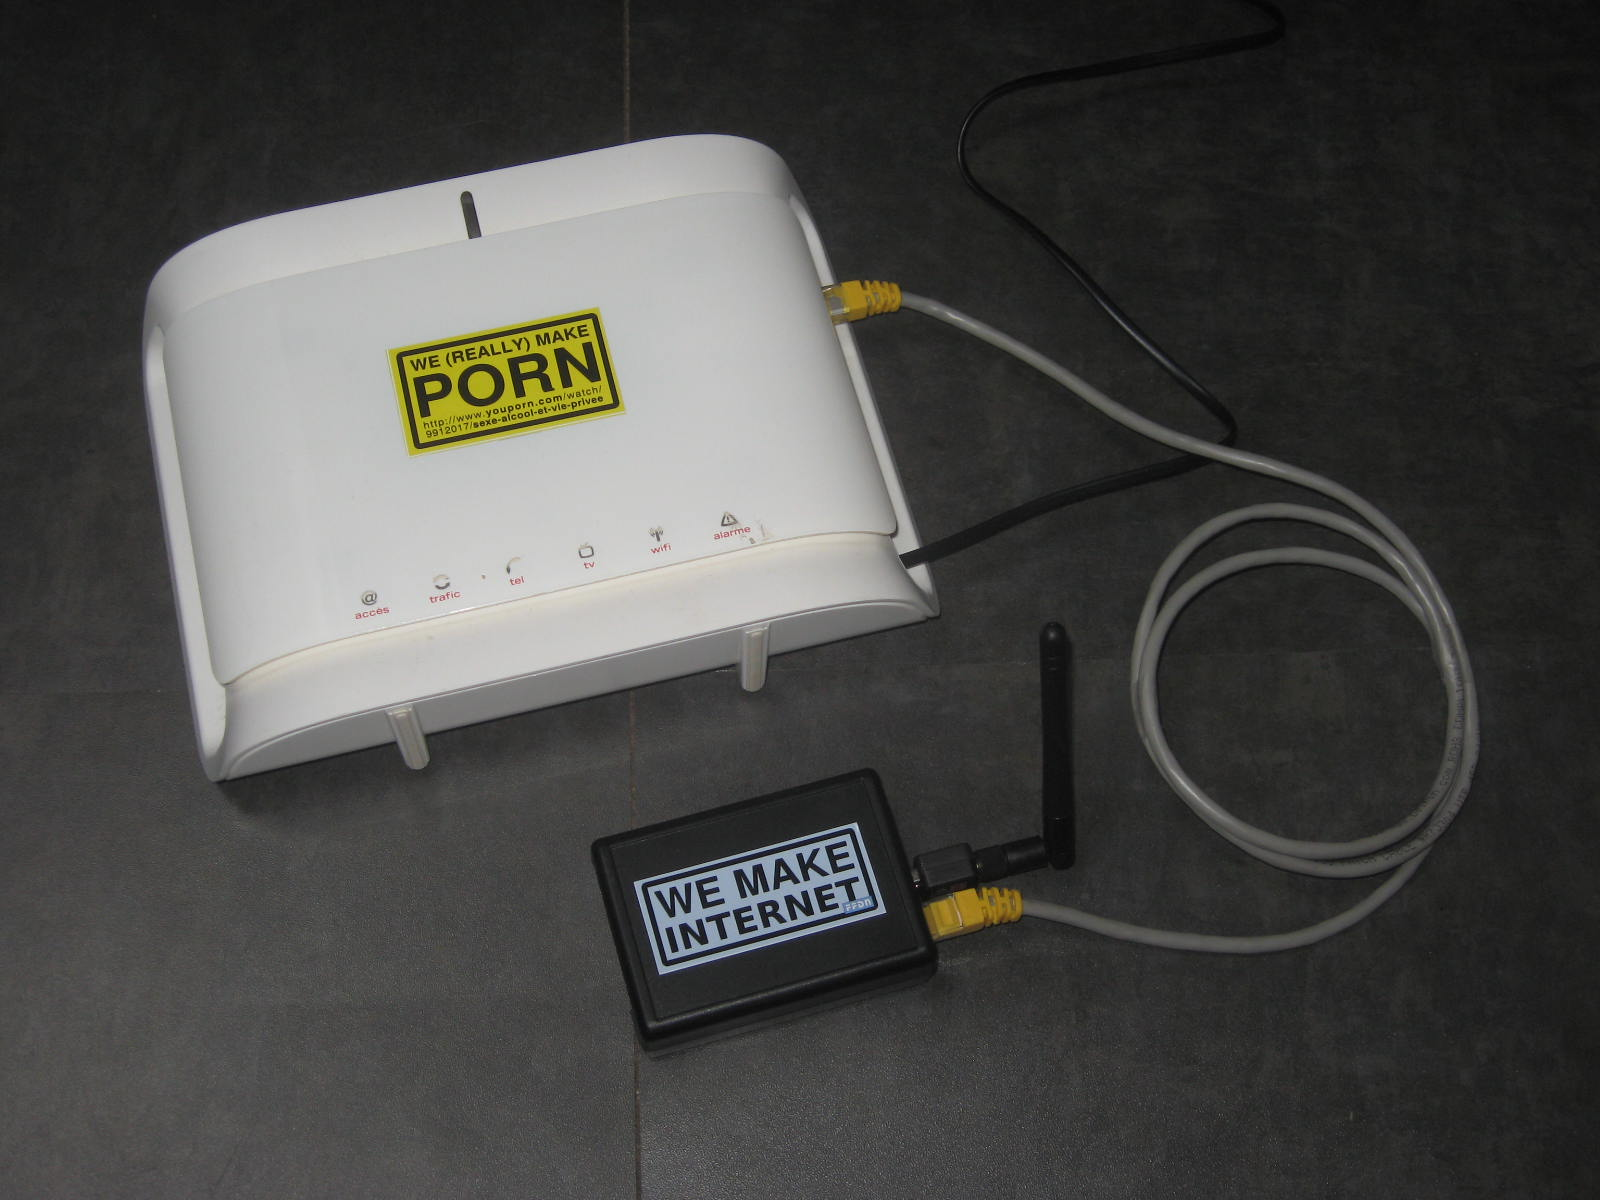
\includegraphics[width=.75\textwidth]{img/05-photo-neufboxboitier.jpg}
\vfill
\end{center}
\end{frame}

\begin{frame}[t]{Et ça marche tout de suite}
\begin{center}
\vfill
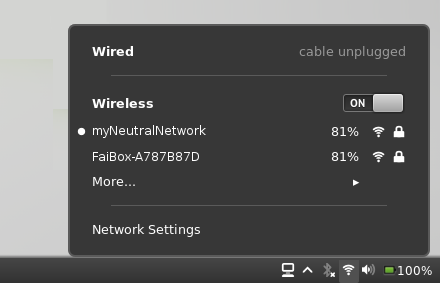
\includegraphics[width=.8\textwidth]{img/06-capture-wifiboitier.png}
\vfill
\end{center}
\end{frame}

\begin{frame}[t]{Mon FAI ne peut plus rien espionner / filtrer / brider}
\begin{center}
\vfill

\includegraphics[width=.9\textwidth]{img/07-schema-connexionboitier.pdf}
\vfill
\end{center}
\end{frame}

\begin{frame}[t]{Sans tunnel VPN}
\begin{center}
\vfill
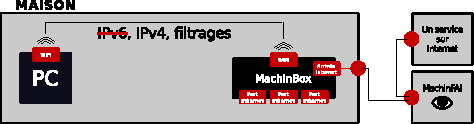
\includegraphics[width=.9\textwidth]{img/schema3.pdf}
\vfill
\end{center}
\end{frame}

\begin{frame}[t]{Avec tunnel VPN}
\begin{center}
\vfill
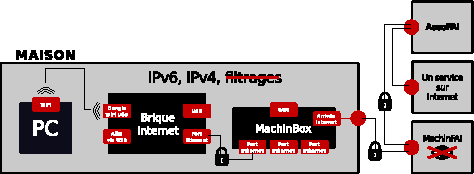
\includegraphics[width=.9\textwidth]{img/schema4.pdf}
\vfill
\end{center}
\end{frame}

%\begin{frame}[t]{Je peux configurer mon Wifi}
%\begin{center}
%\vfill
%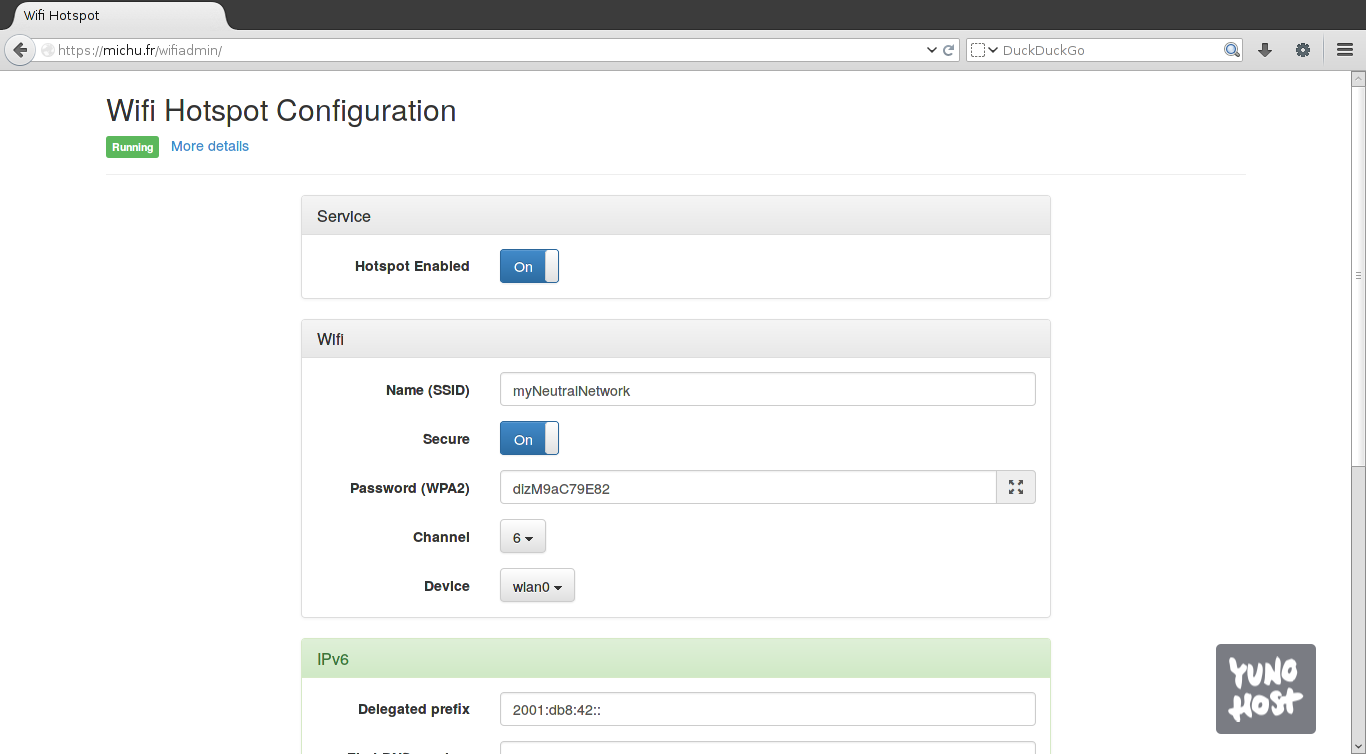
\includegraphics[width=\textwidth]{img/09-capture-wifiadmin.png}
%\vfill
%\end{center}
%\end{frame}

%\begin{frame}[t]{Ou changer d'association}
%\begin{center}
%\vfill
%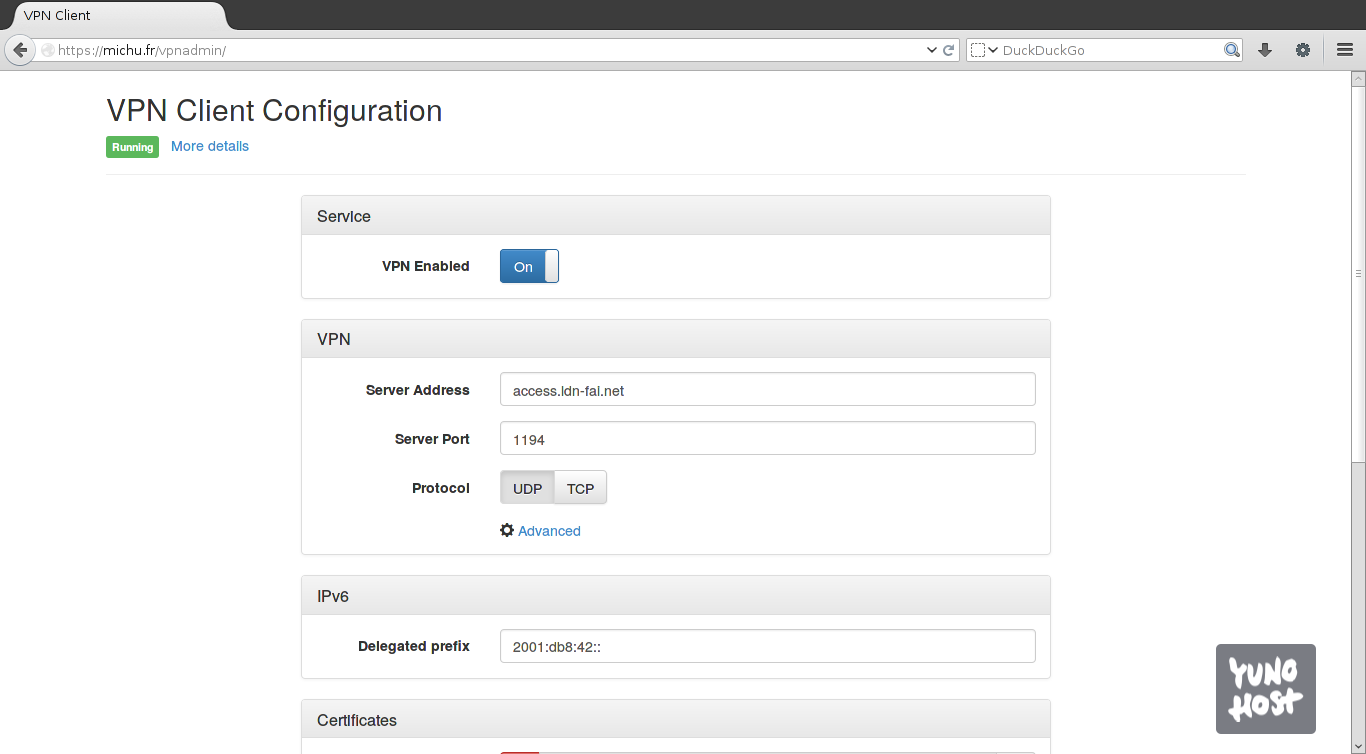
\includegraphics[width=\textwidth]{img/10-capture-vpnadmin.png}
%\vfill
%\end{center}
%\end{frame}

\begin{frame}[t]{Je peux toujours utiliser les autres services de mon FAI}
\begin{center}
\vfill
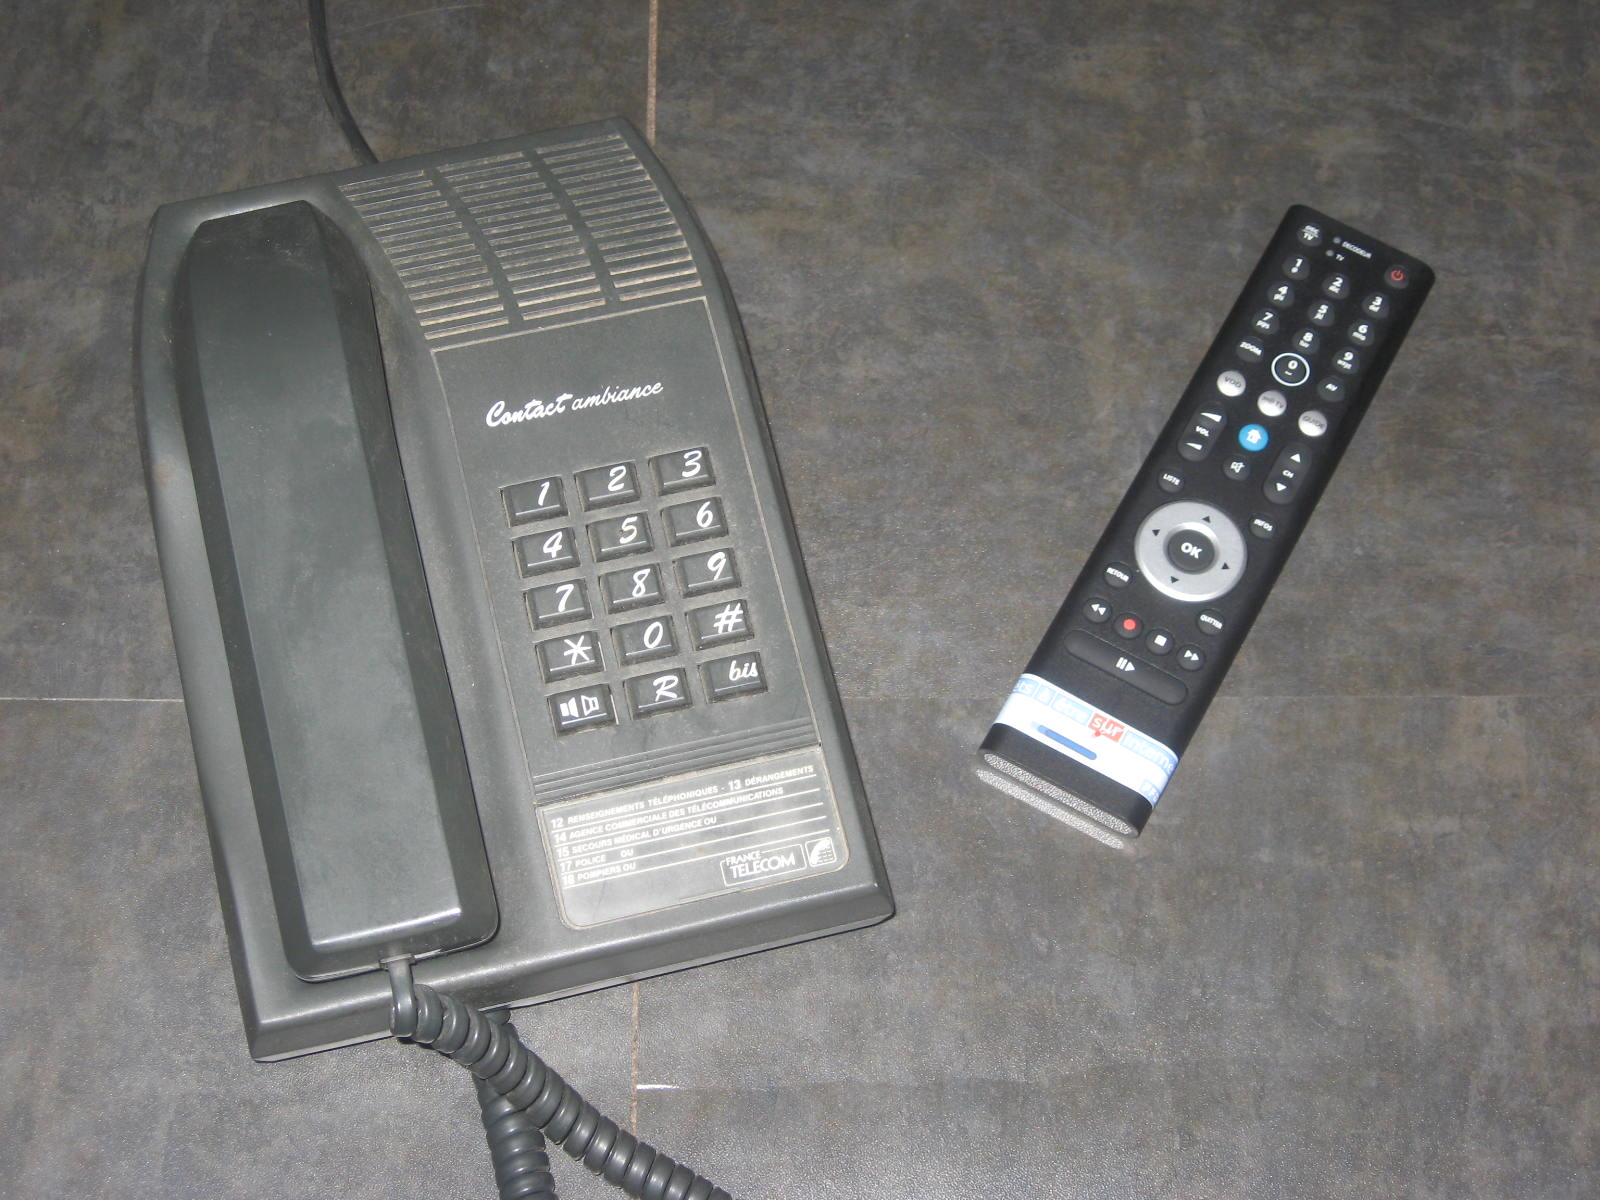
\includegraphics[width=.75\textwidth]{img/13-photo-teltv.jpg}
\vfill
\end{center}
\end{frame}

\begin{frame}[t]{À tout instant je peux changer de Wifi}
\begin{center}
\vfill
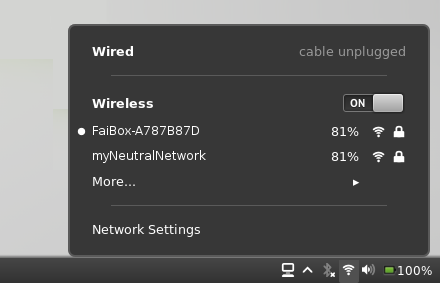
\includegraphics[width=.8\textwidth]{img/14-capture-wifibox2.png}
\vfill
\end{center}
\end{frame}

\begin{frame}[t]{}
\begin{center}
\vfill
{\Huge \textbf{S'auto-héberger}}
\vspace{.5cm}

{\large \emph{En quelques clics}}
\vspace{1cm}

\textbf{2 / 2}
\vfill
\end{center}
\end{frame}

\begin{frame}[t]{Comment communique-t-on sur Internet ?}
\begin{center}
\vfill
\includegraphics[width=.7\textwidth]{img/15a-capture-gmailfbskype.png}
\vfill
\end{center}
\end{frame}

\begin{frame}[t]{Sans tunnel VPN}
\begin{center}
\vfill
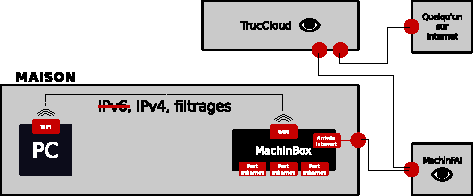
\includegraphics[width=.9\textwidth]{img/schema1.pdf}
\vfill
\end{center}
\end{frame}

\begin{frame}[t]{Avec tunnel VPN}
\begin{center}
\vfill
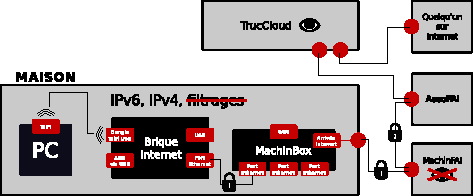
\includegraphics[width=.9\textwidth]{img/schema5.pdf}
\vfill
\end{center}
\end{frame}


\begin{frame}[t]{Ce que vous acceptez chez Google}
	\vspace{4mm}
	\begin{justify}
	« \emph{En soumettant des contenus à nos Services, par importation ou par tout autre moyen, \textbf{vous accordez à Google (et à toute personne travaillant avec Google) une licence}, dans le monde entier, d'utilisation, d'hébergement, de stockage, \textbf{de reproduction, de modification}, de création d’œuvres dérivées [...], de communication, de publication, de représentation publique, \textbf{d'affichage ou de distribution public desdits contenus.}} »\\
	\end{justify}
\end{frame}

%\begin{frame}[t]{Ce que vous acceptez chez Google}
%	\vspace{5mm}
%	\begin{justify}
%	« \emph{Les droits que vous accordez dans le cadre de cette licence \textbf{sont limités à l’exploitation, la promotion ou à l’amélioration de nos Services, ou au développement de nouveaux Services}.} »\\
%	\vspace{5mm}
%	« \emph{Merci d’avoir choisi \textbf{nos produits et services} (les « Services »).} »
%	\end{justify}
%\end{frame}

\begin{frame}[t]{Ce que vous acceptez chez Facebook}
	\vspace{4mm}
	\begin{justify}
	« \emph{Pour le contenu protégé par les droits de propriété intellectuelle, comme les photos ou vidéos, [...] \textbf{vous nous accordez une licence} non-exclusive, \textbf{transférable, sous-licenciable}, sans redevance et mondiale \textbf{pour l'utilisation des contenus de propriété intellectuelle que vous publiez} sur Facebook ou en relation à Facebook} »
	\end{justify}
\end{frame}

\begin{frame}[t]{Pendant combien de temps chez Google}
	\vfill
	\begin{justify}
	« \emph{Cette autorisation demeure pour toute la durée légale de protection de votre contenu, \textbf{même si vous cessez d’utiliser nos Services}.} »
	\end{justify}
	\vfill
\end{frame}

\begin{frame}[t]{Pendant combien de temps chez Facebook}
	\vspace{4mm}
	\begin{justify}
	« \emph{Cette licence de propriété intellectuelle \textbf{se termine lorsque vous supprimez vos contenus} de propriété intellectuelle ou votre compte, \textbf{sauf si votre compte est partagé avec d'autres personnes} qui ne l'ont pas supprimé.} »\\

	\vspace{4mm}
	« \emph{Lorsque vous supprimez votre contenu [...], vous comprenez que \textbf{les contenus supprimés peuvent persister dans des copies} de sauvegarde pendant \textbf{un certain temps}.} »
	\end{justify}
\end{frame}


\begin{frame}[t]{Un très bon endroit pour les stocker, c'est chez soi}
\begin{center}
\vfill
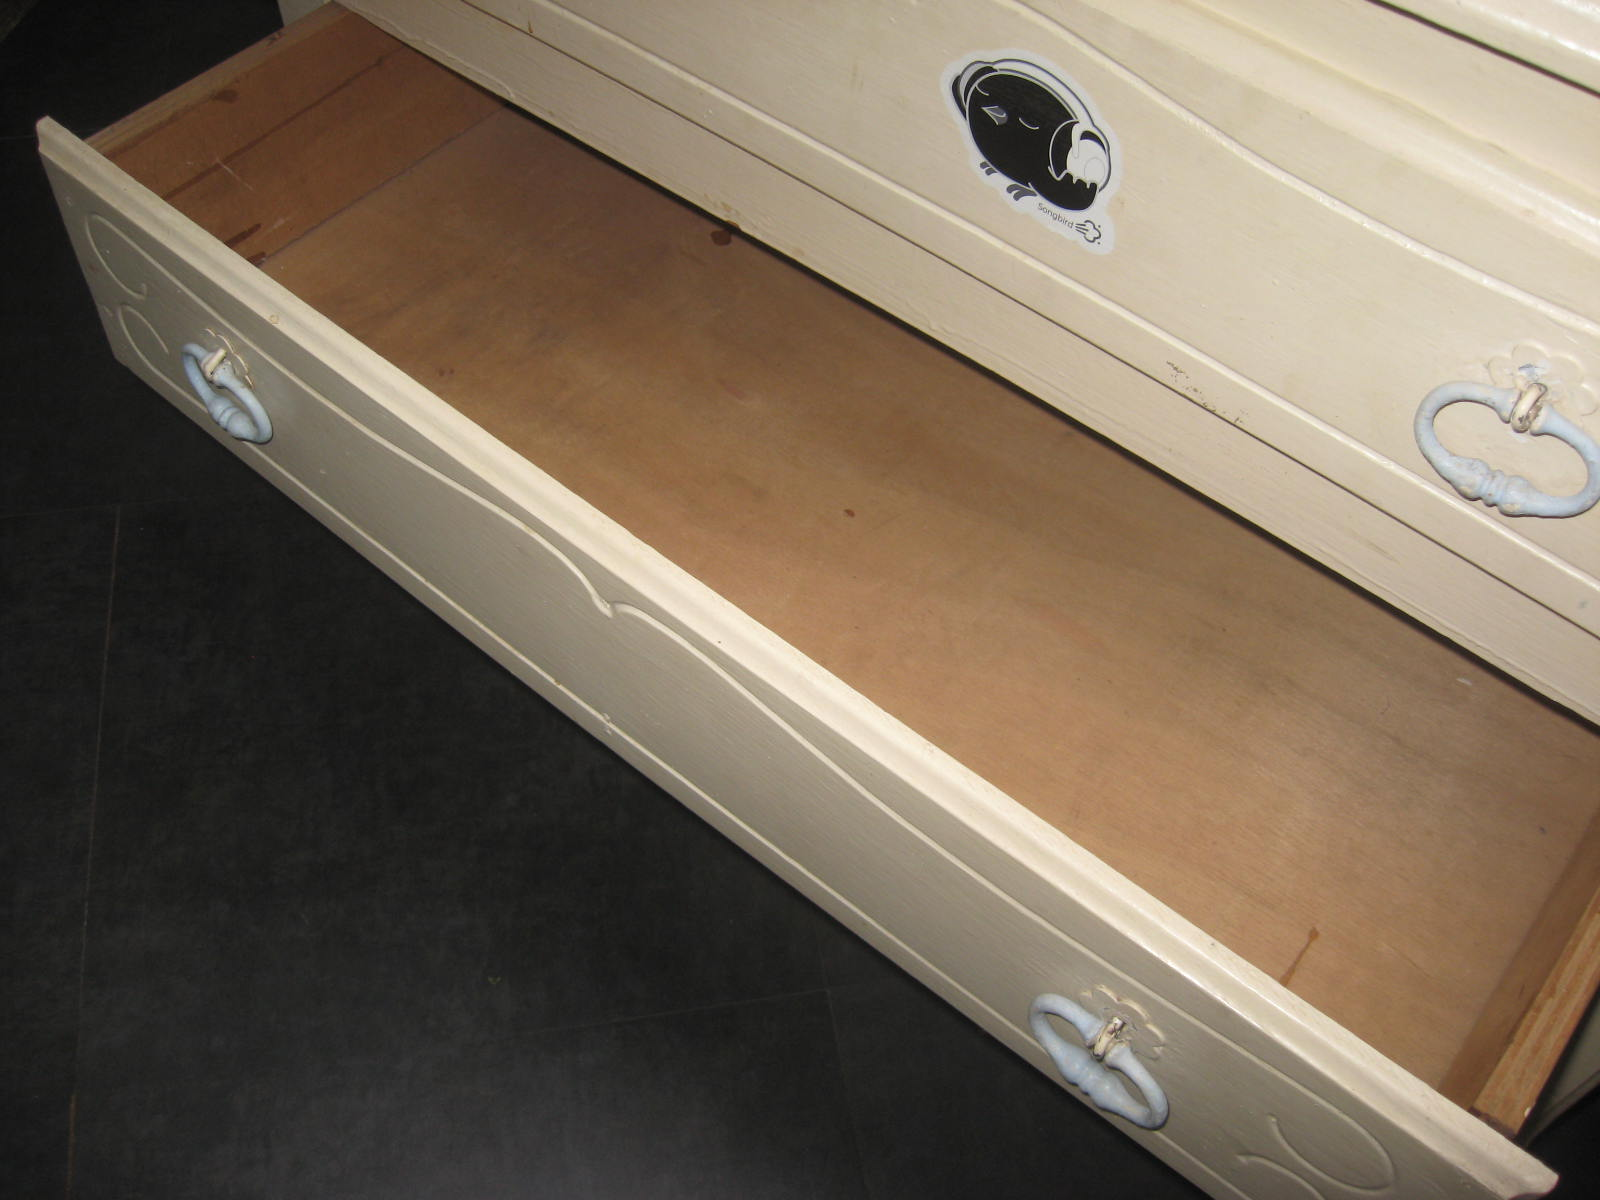
\includegraphics[width=.75\textwidth]{img/15b-photo-commode.jpg}
\vfill
\end{center}
\end{frame}

\begin{frame}[t]{La Brique Internet permet aussi de faire ça !}
\begin{center}
\vfill
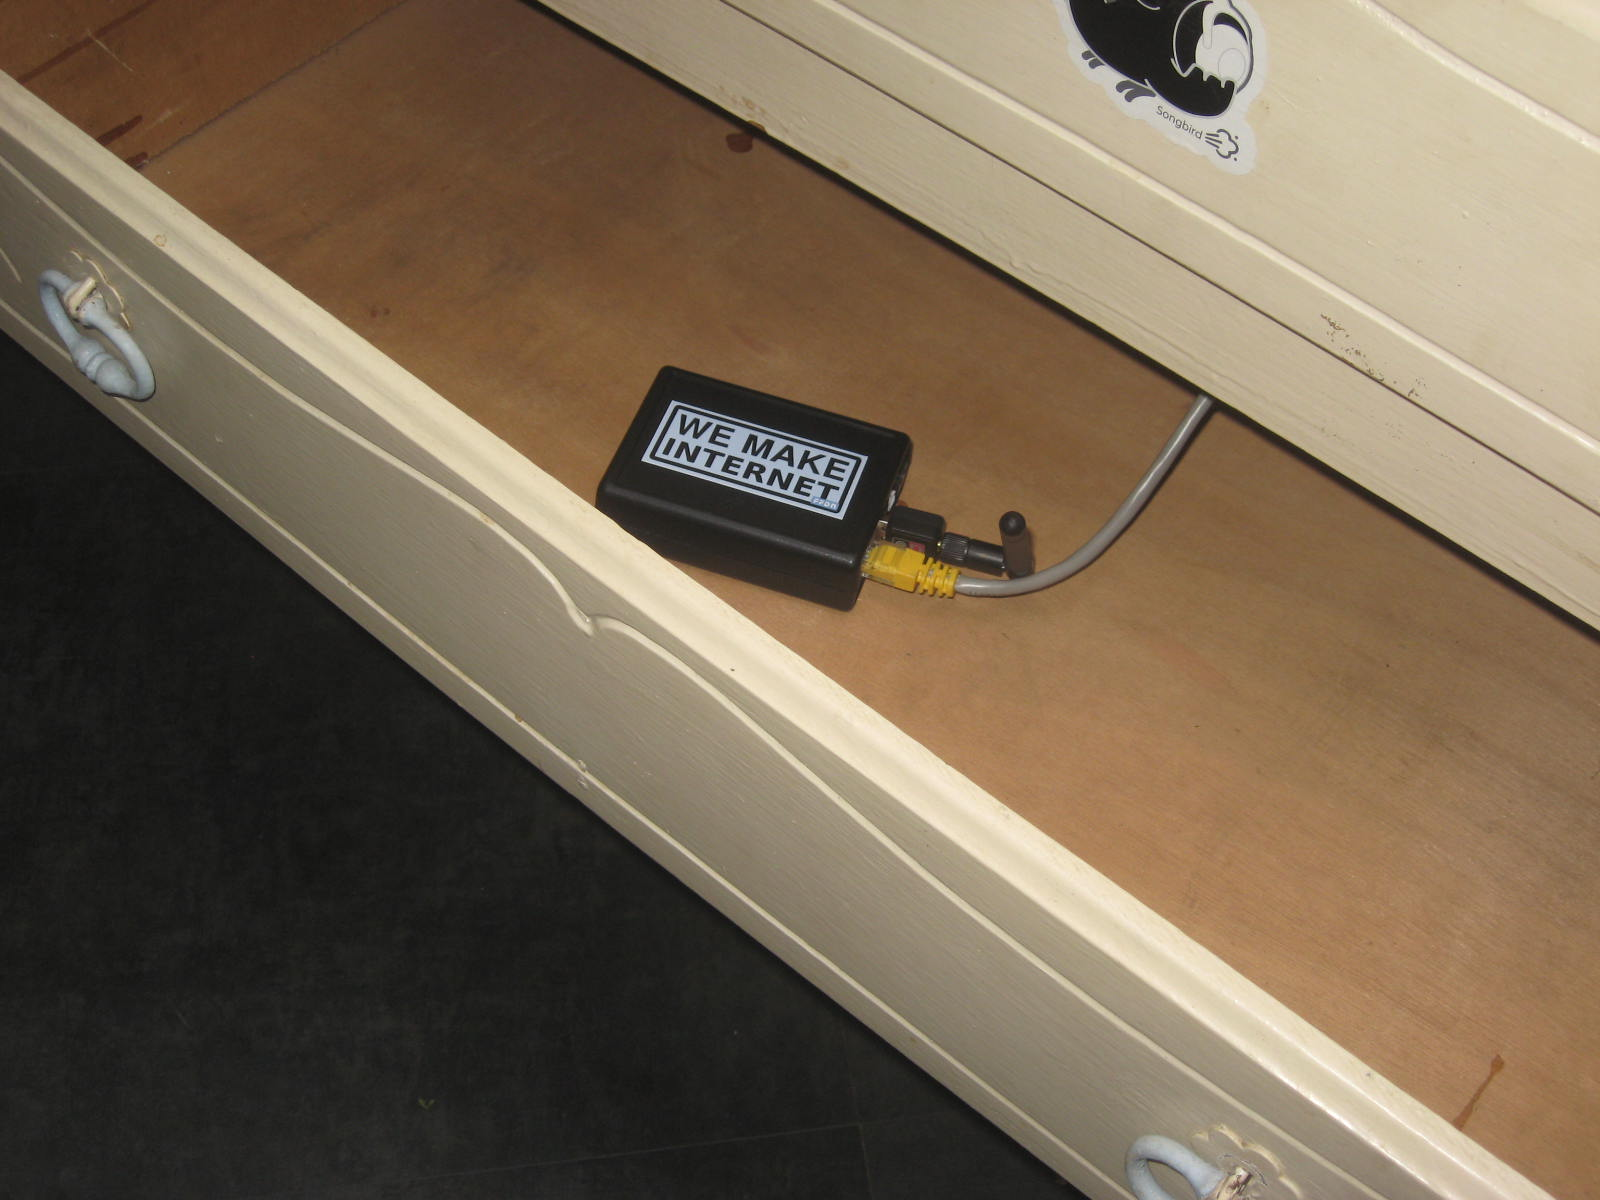
\includegraphics[width=.75\textwidth]{img/16-photo-boitiercommode.jpg}
\vfill
\end{center}
\end{frame}

\begin{frame}[t]{Grâce à YunoHost}
\begin{center}
\vfill
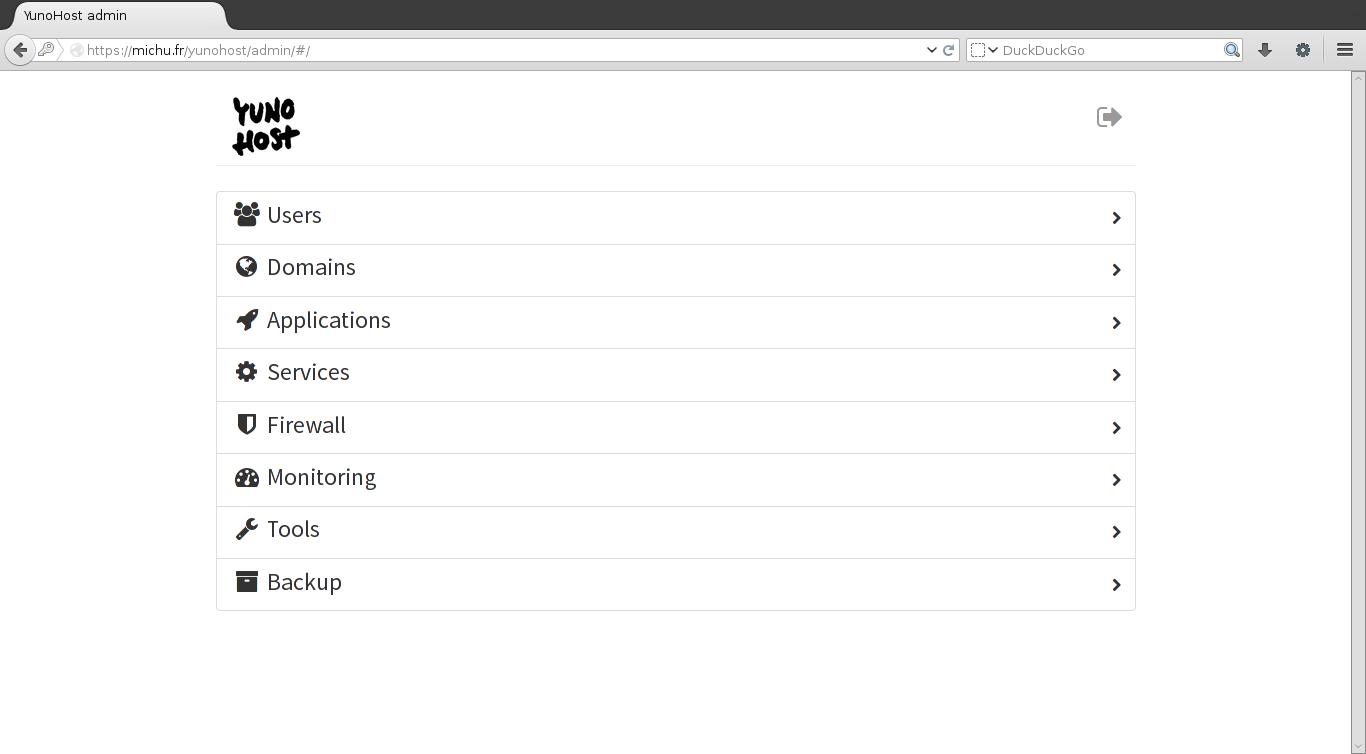
\includegraphics[width=\textwidth]{img/17a-capture-yunohost.png}
\vfill
\end{center}
\end{frame}

%\begin{frame}[t]{Je peux par exemple installer mon webmail}
%\begin{center}
%\vfill
%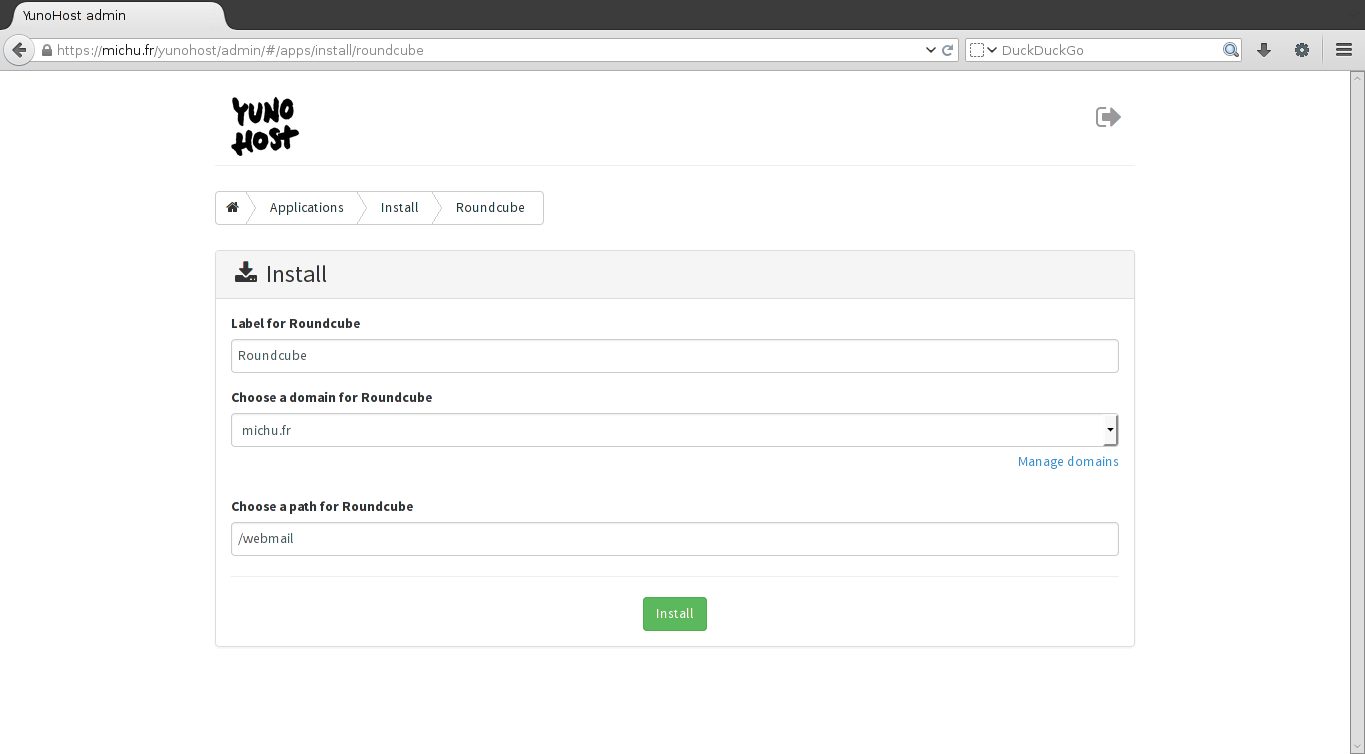
\includegraphics[width=\textwidth]{img/17b-capture-installroundcube.png}
%\vfill
%\end{center}
%\end{frame}
%
%\begin{frame}[t]{Et c'est immédiatement accessible}
%\begin{center}
%\vfill
%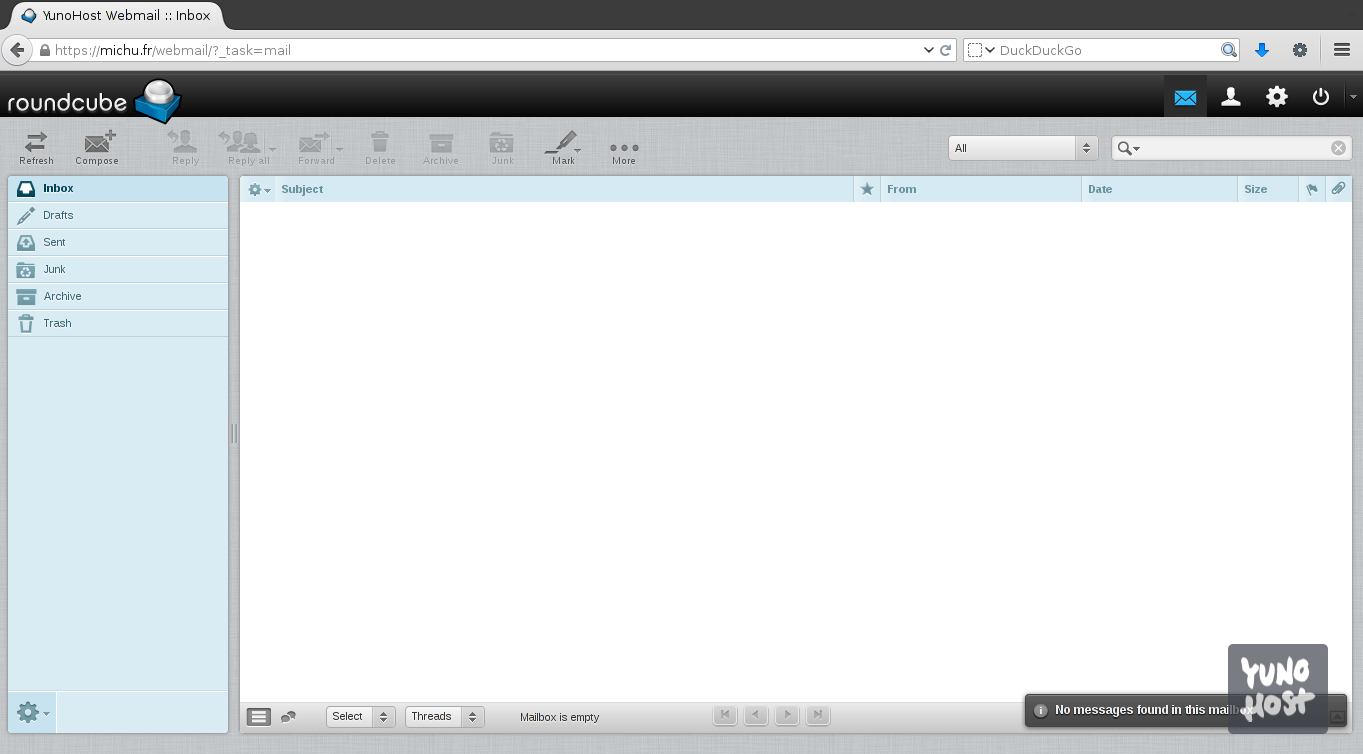
\includegraphics[width=\textwidth]{img/18-capture-roundcube.png}
%\vfill
%\end{center}
%\end{frame}

\begin{frame}[t]{Avec plein d'applications à installer}
\begin{center}
\vfill
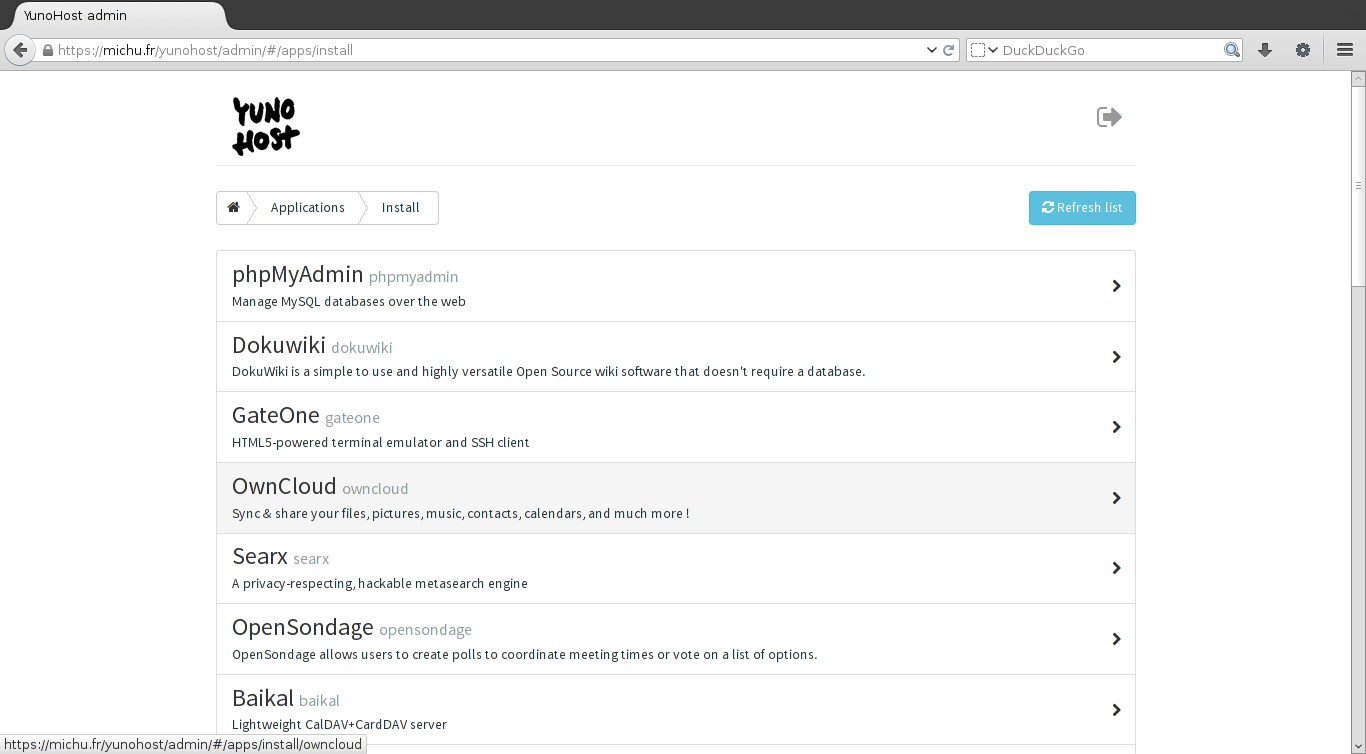
\includegraphics[width=\textwidth]{img/19-capture-yunohostapps.png}
\vfill
\end{center}
\end{frame}

%\begin{frame}[t]{Les interfaces Wifi \& VPN sont des applications}
%\begin{center}
%\vfill
%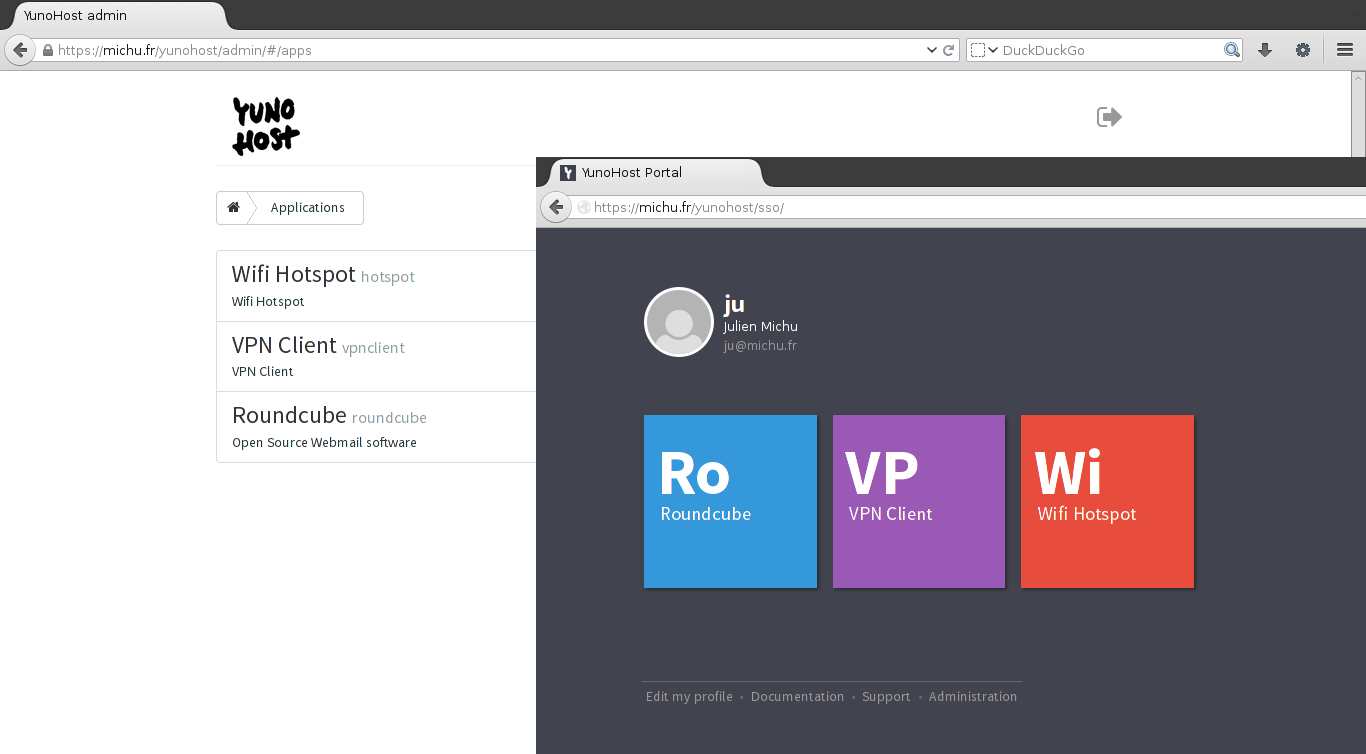
\includegraphics[width=\textwidth]{img/20-capture-yunohostinstalled.png}
%\vfill
%\end{center}
%\end{frame}

\begin{frame}[t]{Avec la Brique Internet}
\begin{center}
\vfill
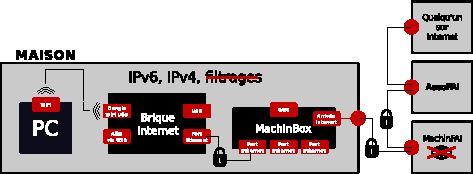
\includegraphics[width=.9\textwidth]{img/schema2.pdf}
\vfill
\end{center}
\end{frame}


\begin{frame}[t]{}
\begin{center}
\vfill
{\Huge \textbf{Où trouver ce boîtier ?}}
\vspace{.5cm}

{\large \emph{Parce qu'il n'y en a pas à Carrefour}}
\vfill
\end{center}
\end{frame}

\begin{frame}[t]{Dans des associations locales}
\begin{center}
\vfill
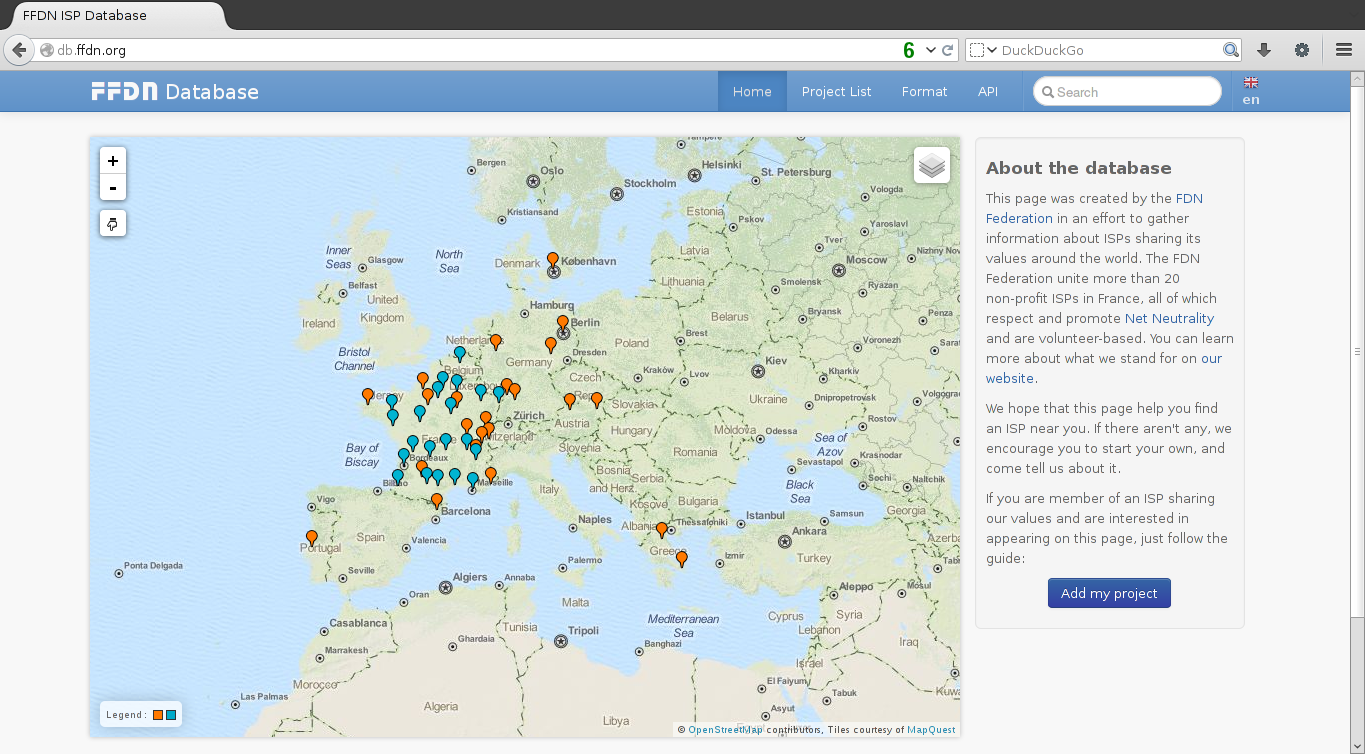
\includegraphics[width=\textwidth]{img/25a-capture-ffdn.png}
\vfill
\end{center}
\end{frame}

\begin{frame}[t]{Ou le faire soi-même, puisque tout est libre}
\begin{center}
\vfill
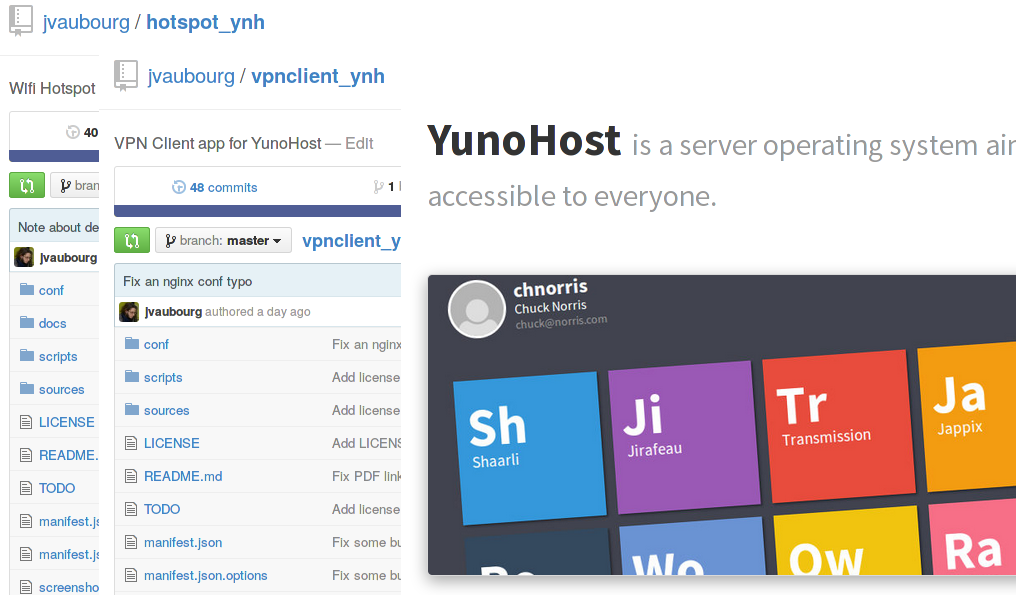
\includegraphics[width=\textwidth]{img/25b-capture-github.png}
\vfill
\end{center}
\end{frame}

\begin{frame}[t]{}
\begin{center}
\vfill
\vfill
{\Large Environ \textbf{70\euro{} pour 1 Brique$^*$} complète \\ (frais de port inclus)}
\vspace{1cm}

{\Large Environ \textbf{7 \euro{} / mois} pour un \\ \textbf{accès VPN} associatif}
\vspace{1cm}
\vfill

{\footnotesize \emph{* pour une commande groupée > 9 Briques, sinon 80\euro}}
\vfill
\end{center}
\end{frame}

\begin{frame}[t]{}
\begin{center}
\vfill
{\Huge \textbf{Bonus}}
\vspace{.5cm}

{\large \emph{Encore, encore !}}
\vfill
\end{center}
\end{frame}

%\begin{frame}[t]{Si je change de FAI}
%\begin{center}
%\vfill
%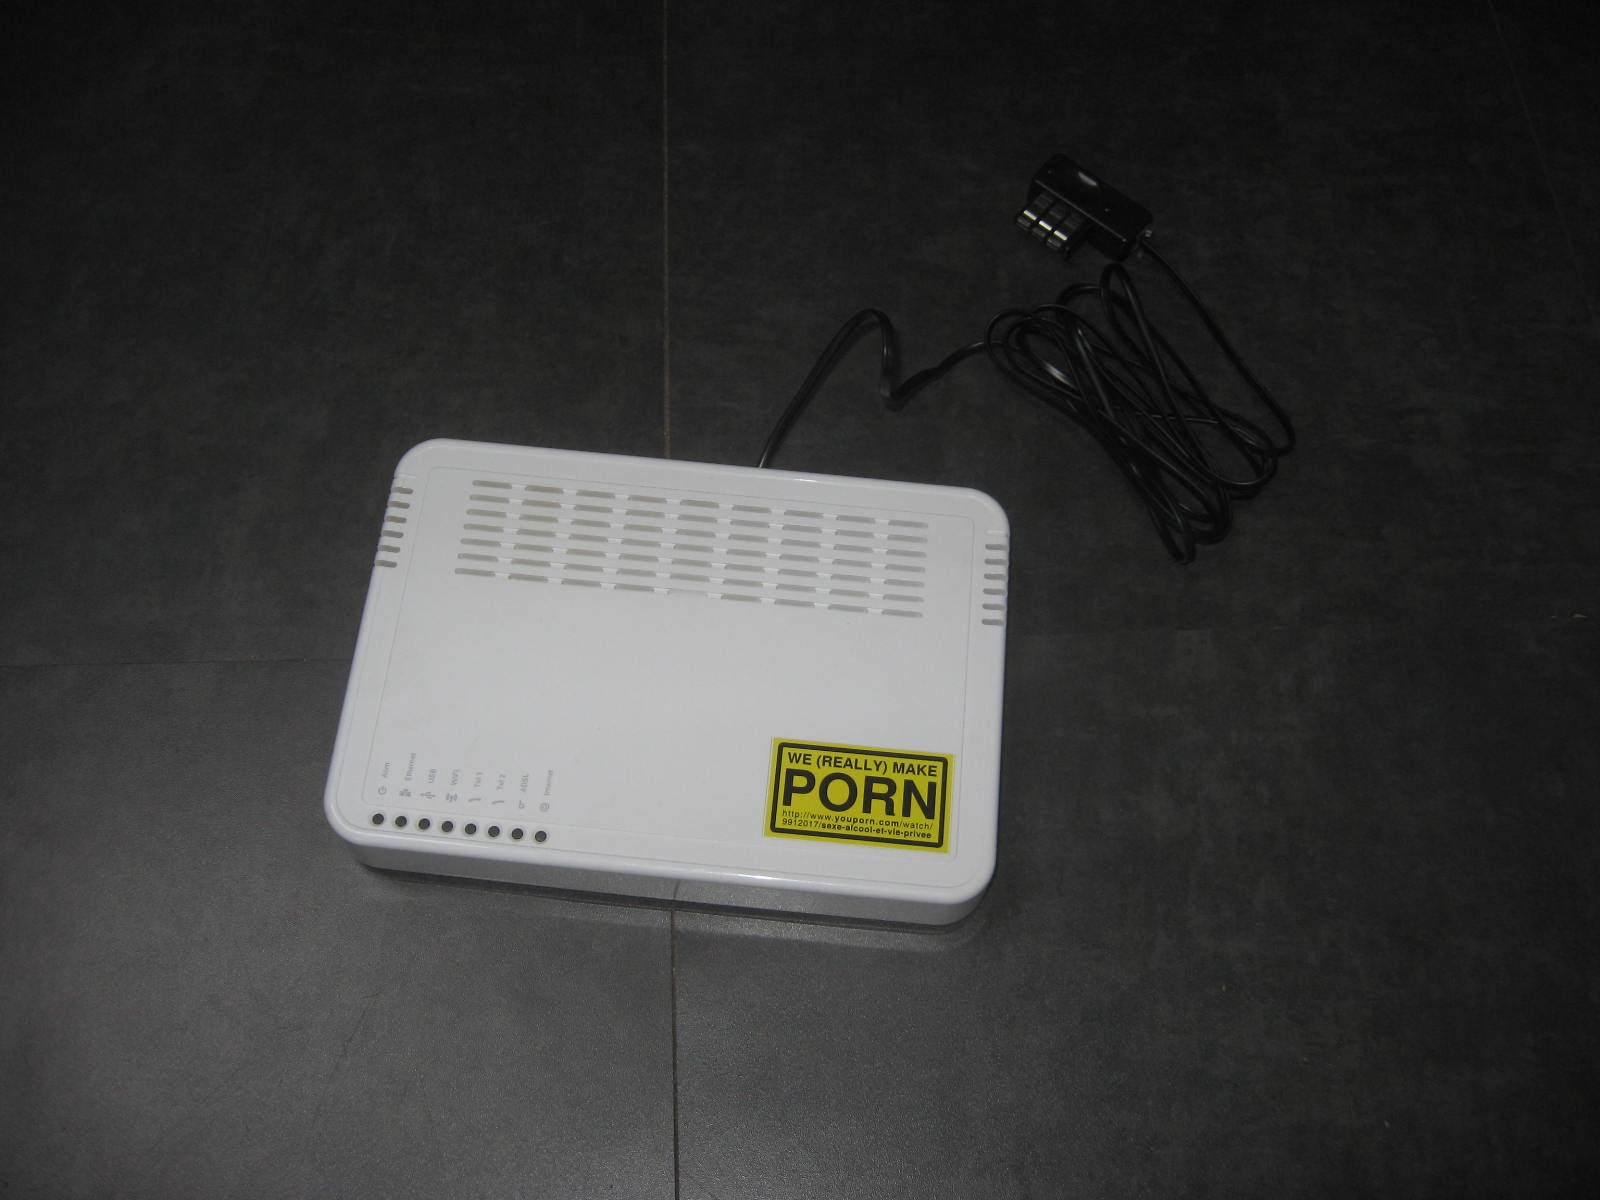
\includegraphics[width=.75\textwidth]{img/11a-photo-bbox.jpg}
%\vfill
%\end{center}
%\end{frame}

%\begin{frame}[t]{Je n'ai qu'à débrancher et rebrancher ma Brique}
%\begin{center}
%\vfill
%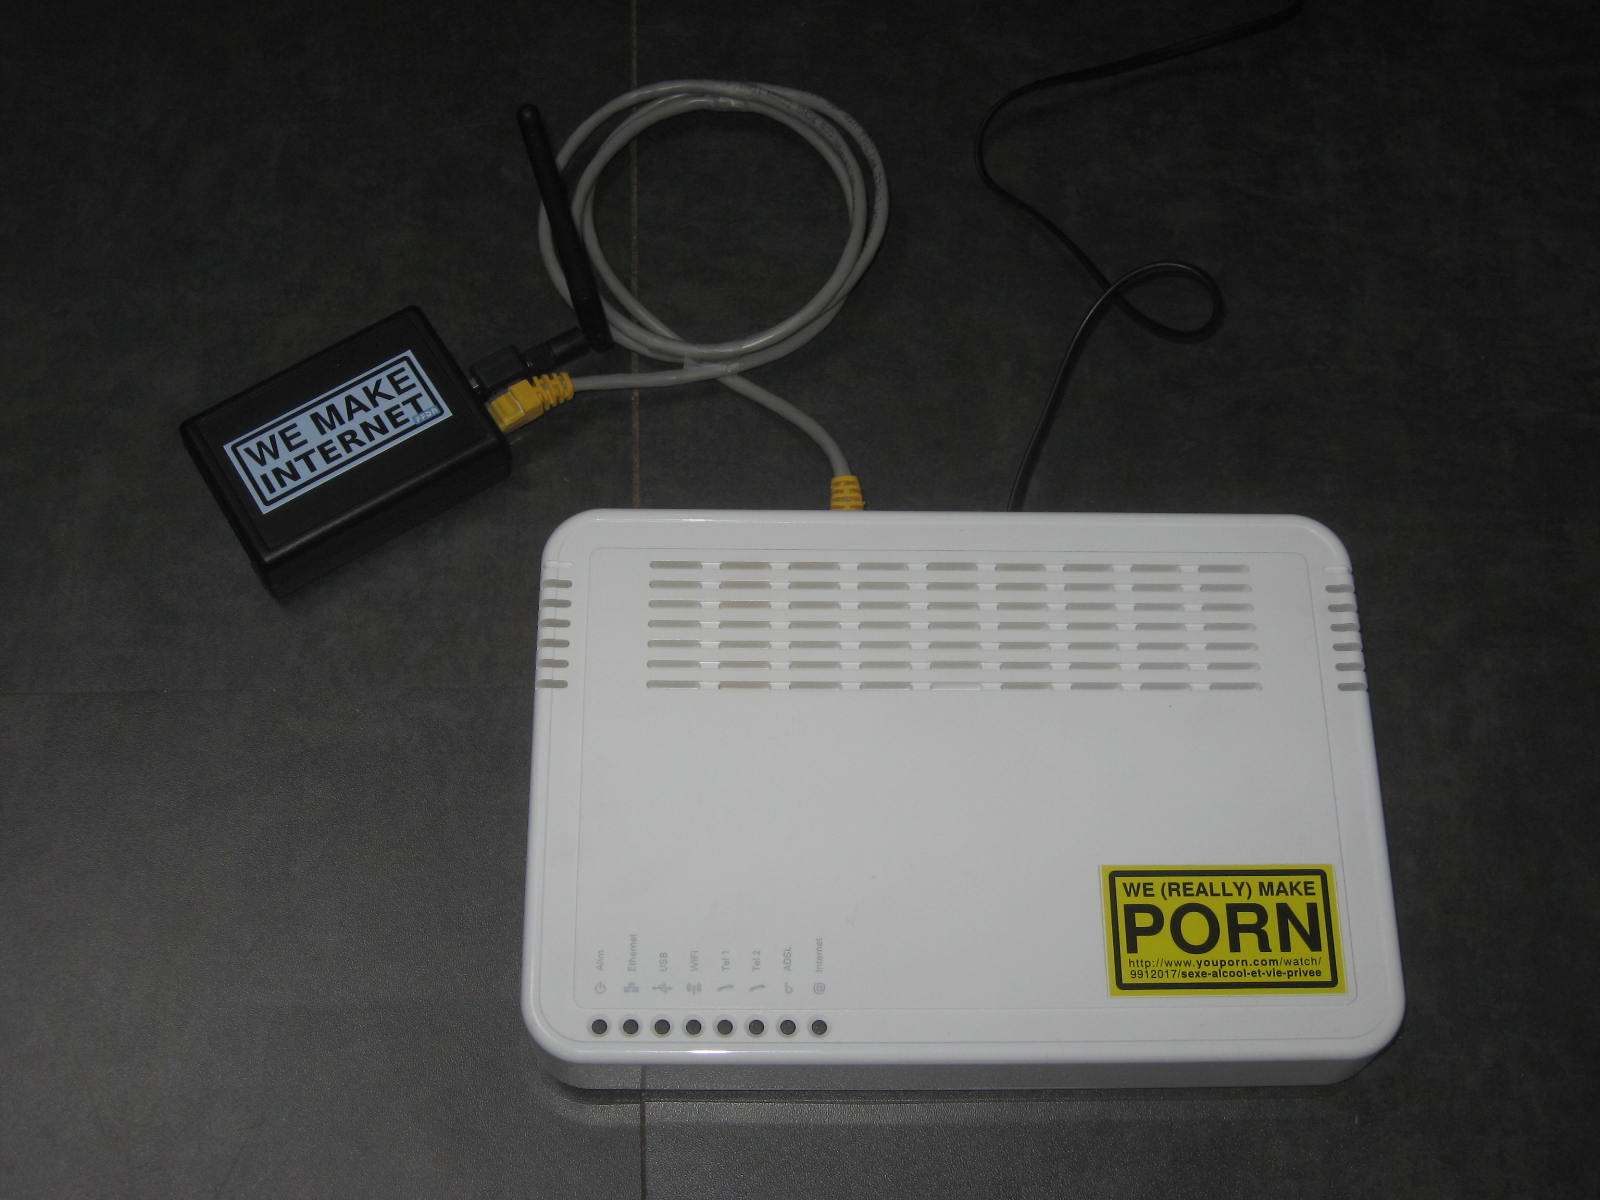
\includegraphics[width=.75\textwidth]{img/11b-photo-bboxboitier.jpg}
%\vfill
%\end{center}
%\end{frame}

\begin{frame}[t]{Je peux déménager ou changer de FAI sans problème}
\begin{center}
\vfill
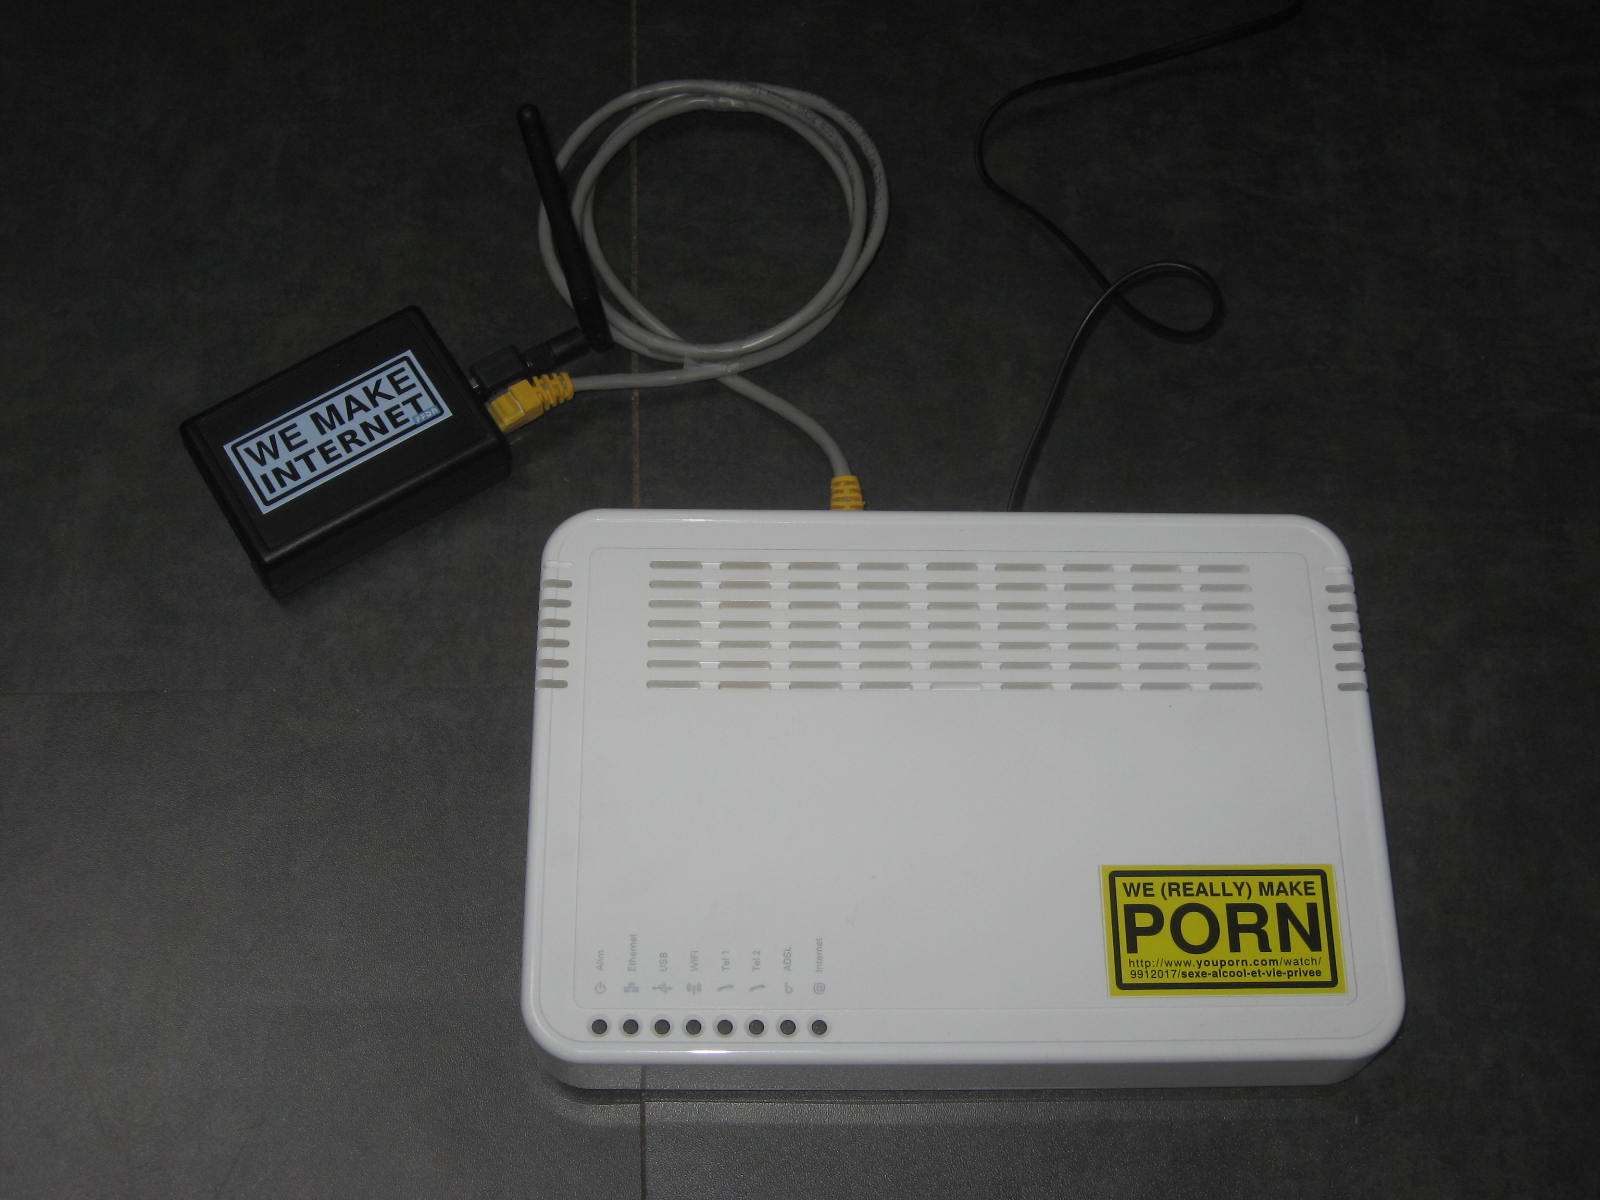
\includegraphics[width=.75\textwidth]{img/21-photo-bboxboitier.jpg}
\vfill
\end{center}
\end{frame}

\begin{frame}[t]{Il suffit de débrancher/rebrancher la Brique}
\begin{center}
\vfill
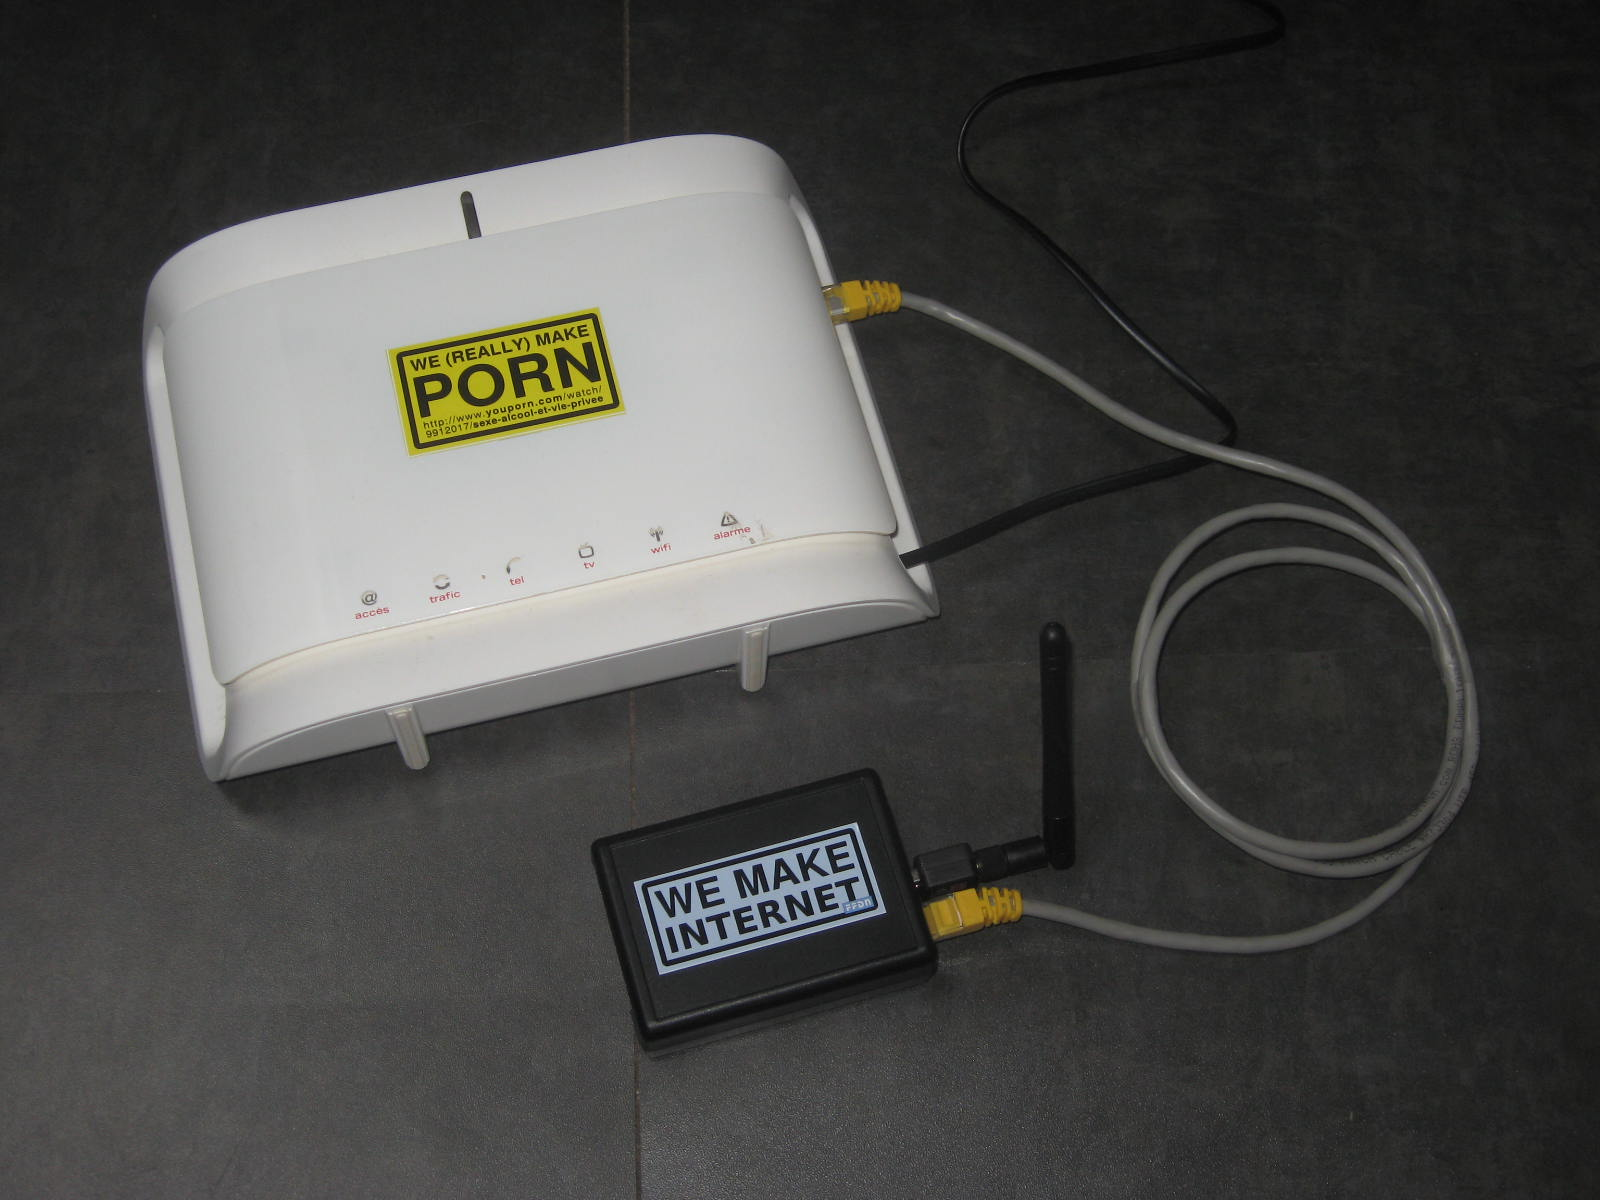
\includegraphics[width=.75\textwidth]{img/22-photo-neufboxboitier.jpg}
\vfill
\end{center}
\end{frame}

\begin{frame}[t]{Et ça marche toujours sans rien reconfigurer}
\begin{center}
\vfill
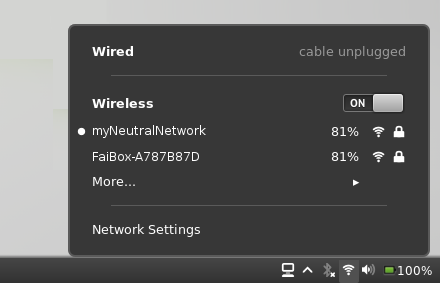
\includegraphics[width=.8\textwidth]{img/12-capture-wifiboitier2.png}
\vfill
\end{center}
\end{frame}



\begin{frame}[t]{Y compris sur un accès très filtré}
\begin{center}
\vfill
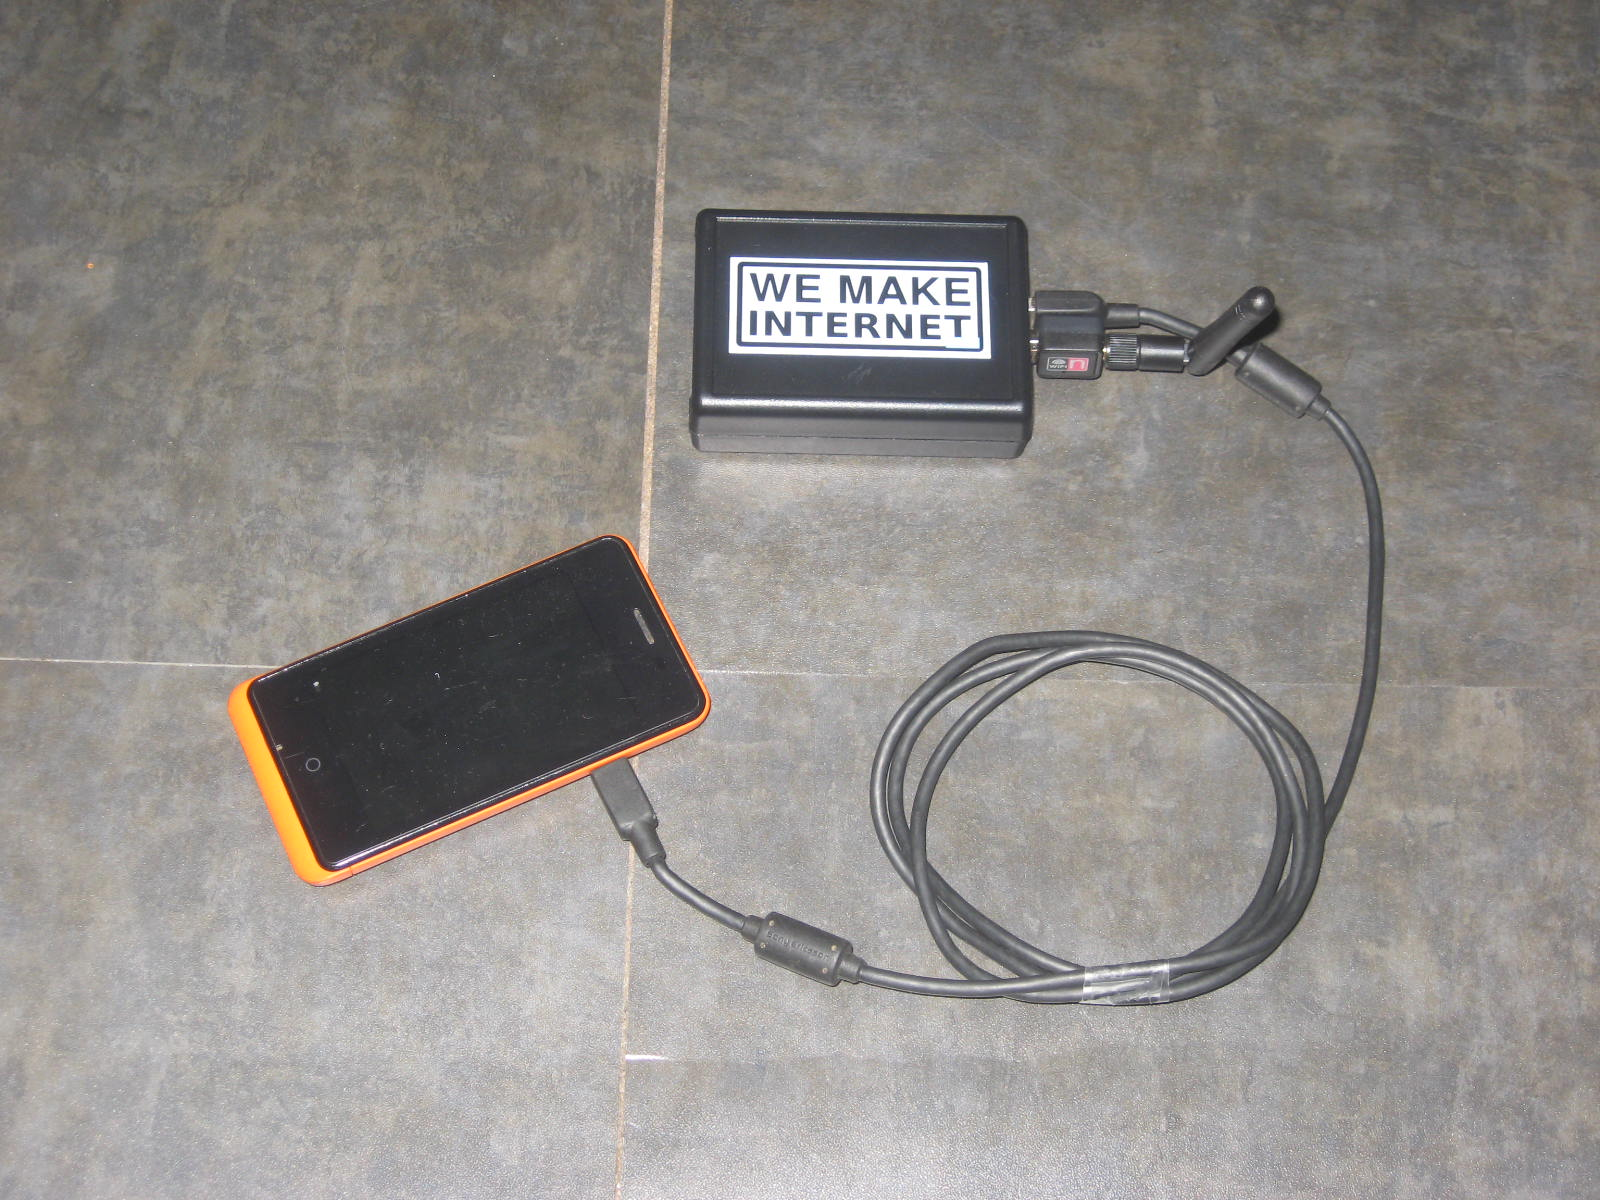
\includegraphics[width=.75\textwidth]{img/23-photo-boitier3g.jpg}
\vfill
\end{center}
\end{frame}



%\begin{frame}[t]{Je peux détourner l'usage de la Brique}
%\begin{center}
%\vfill
%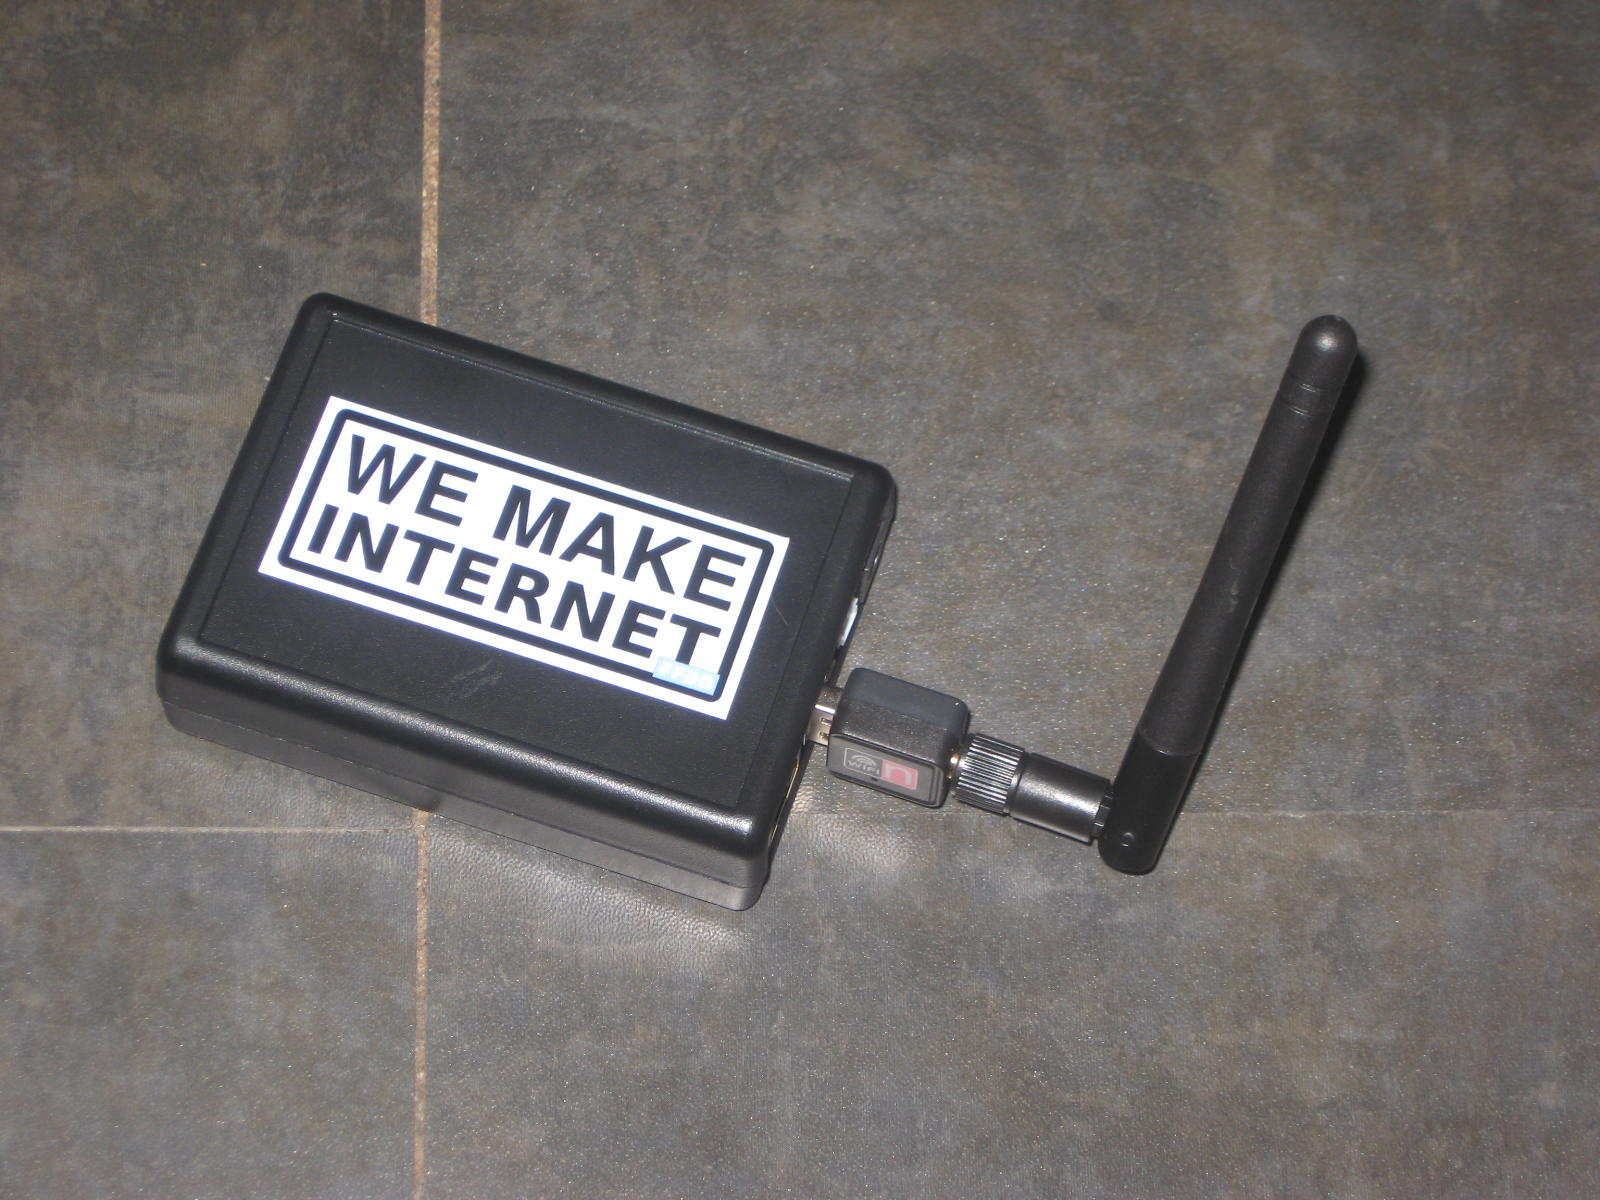
\includegraphics[width=.75\textwidth]{img/27-photo-boitier.jpg}
%\vfill
%\end{center}
%\end{frame}

\begin{frame}[t]{Je peux l'utiliser pour en faire une PirateBox}
\begin{center}
\vfill
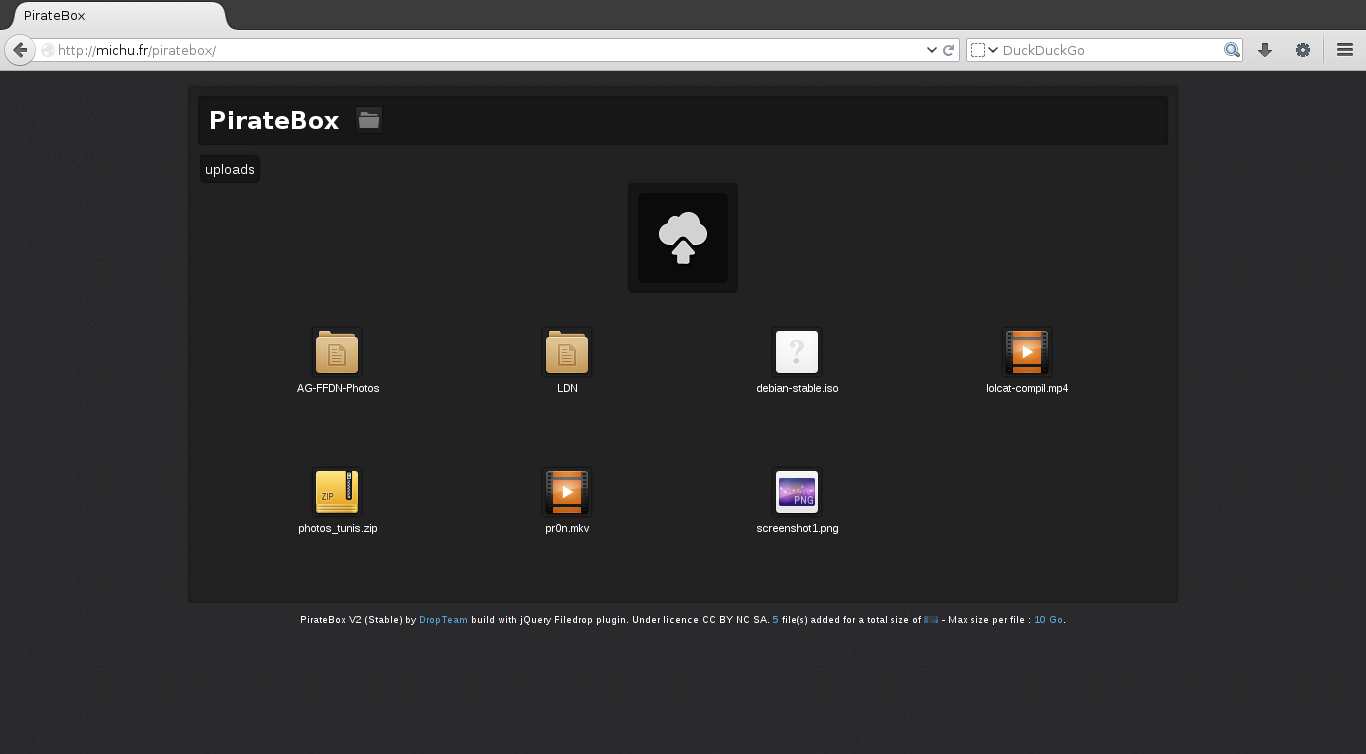
\includegraphics[width=\textwidth]{img/28-capture-piratebox.png}
\vfill
\end{center}
\end{frame}

%\begin{frame}[t]{Je peux aussi couvrir un événement public}
%\begin{center}
%\vfill
%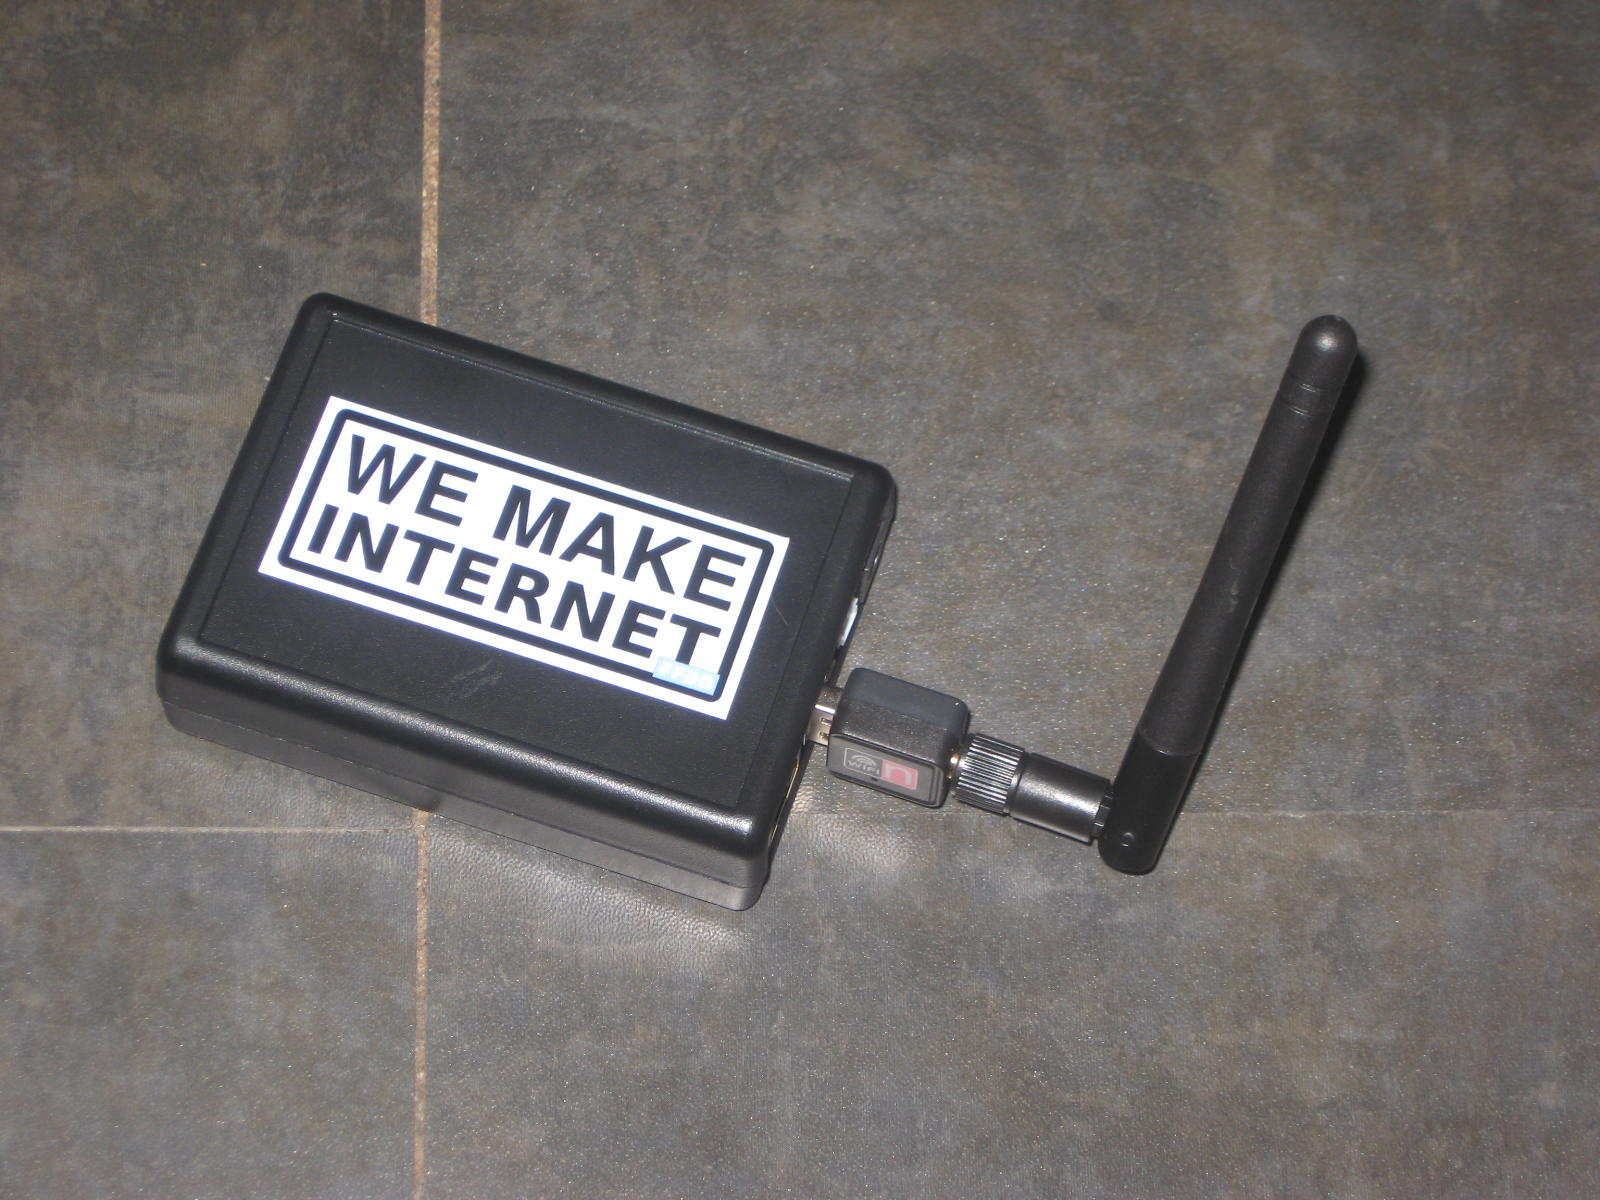
\includegraphics[width=.75\textwidth]{img/27-photo-boitier.jpg}
%\vfill
%\end{center}
%\end{frame}

\begin{frame}[t]{J'ai accès à de l'IPv6}
\begin{center}
\vfill
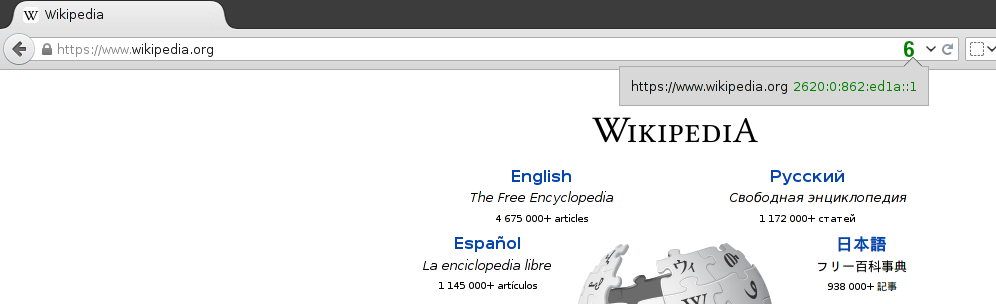
\includegraphics[width=\textwidth]{img/08-capture-ipv6wikipedia.png}
\vfill
\end{center}
\end{frame}

\begin{frame}[t]{Et mes services sont accessibles en IPv6}
\begin{center}
\vfill
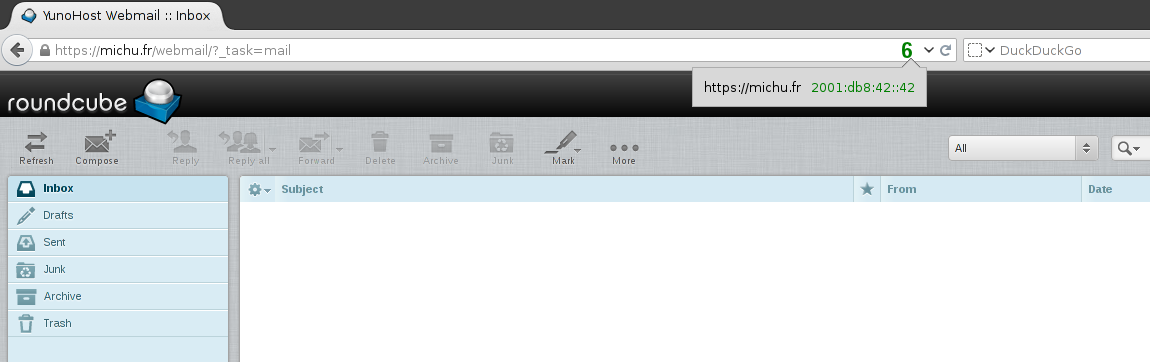
\includegraphics[width=\textwidth]{img/24-capture-ipv6roundcube.png}
\vfill
\end{center}
\end{frame}

\begin{frame}[t]{La Brique Internet, c'est :}
\vfill
\begin{itemize}
\item \textbf{s'émanciper} du pouvoir de son FAI \vfill
\item \textbf{reprendre le contrôle} de ses données \vfill
\item \textbf{utiliser Internet} sereinement
\end{itemize}
\vfill
\end{frame}

\begin{frame}[t]{}
\begin{center}
\vfill
\vspace{.5cm}

{\Huge LaBriqueInter.net}
\vspace{1.5cm}

Trouver une association près de chez vous :
\vspace{.5cm}

{\Large \url{db.ffdn.org}}
\vfill
\end{center}
\end{frame}


\end{document}
